% --------------------------------------
% Master's Thesis Title Page
% LaTeX Template
% Version 1.0 (23/05/14)
% Thanks to Magnus Marthinsen, this thesis and template is made available for Master studentes at HVL Joint SE program (01.03.2021)
%---------------------------------------

%----------------------------------------------------------------------------------------
%	PACKAGES AND OTHER DOCUMENT CONFIGURATIONS
%----------------------------------------------------------------------------------------
\documentclass[a4paper]{report}
\usepackage{graphicx} % Required for box manipulation
\usepackage{helvet}
\usepackage{subfig}
\usepackage[utf8]{inputenc}
%\usepackage{natbib}
\usepackage[USenglish]{babel}
\usepackage[useregional]{datetime2}
\usepackage{pgfgantt}
\usepackage{listings}
\usepackage{wrapfig}
\usepackage{setspace}
\usepackage{parskip} % Used to create spaces between paragraphs
\usepackage{dirtytalk} % quotes by talk
\usepackage[hidelinks]{hyperref}
% \usepackage[acronym, toc]{glossaries}  % Used to add a wordlist/glossaries
\usepackage{mathtools}
\usepackage{amsfonts}
\usepackage{color, colortbl}
\usepackage{booktabs}
\usepackage{float}
\usepackage{csquotes}

%BIB by Adrian
\usepackage[backend=biber,style=numeric, urldate=long]{biblatex}
% See the references.bib file. Most Bibtex bibliographies in Computer Science can be found from dblp.org
\addbibresource{report.bib}



% Glossary/wordlist
% \makeglossaries
% \input{glossaries.tex}

\begin{document}

%
% COLORS USED THROUGH THE REPORT
%
\definecolor{kb_red}{RGB}{96,2,4}
\definecolor{light_gray}{RGB}{160,160,160}
\definecolor{med_gray}{RGB}{96,94,94}
\definecolor{black}{RGB}{0,0,0}
\definecolor{white}{RGB}{155,155,155}
\definecolor{light_green}{RGB}{208,240,192}
\definecolor{light_red}{RGB}{255,204,203}

% CODE STYLE
\definecolor{javared}{rgb}{0.6,0,0} % for strings
\definecolor{javagreen}{rgb}{0.25,0.5,0.35} % comments
\definecolor{javapurple}{rgb}{0.5,0,0.35} % keywords
\definecolor{javadocblue}{rgb}{0.25,0.35,0.75} % javadoc

\makeatletter
\lst@Key{matchrangestart}{f}{\lstKV@SetIf{#1}\lst@ifmatchrangestart}
\def\lst@SkipToFirst{%
    \lst@ifmatchrangestart\c@lstnumber=\numexpr-1+\lst@firstline\fi
    \ifnum \lst@lineno<\lst@firstline
        \def\lst@next{\lst@BeginDropInput\lst@Pmode
        \lst@Let{13}\lst@MSkipToFirst
        \lst@Let{10}\lst@MSkipToFirst}%
        \expandafter\lst@next
    \else
        \expandafter\lst@BOLGobble
    \fi}
\makeatother

\lstset{language=Java,
basicstyle=\footnotesize,
keywordstyle=\color{javapurple}\bfseries,
stringstyle=\color{javared},
commentstyle=\color{javagreen},
morecomment=[s][\color{javadocblue}]{/**}{*/},
numbers=left,
captionpos=b,
frame=single,
breakatwhitespace=false,
breaklines=true,
numberstyle=\tiny\color{black},
stepnumber=1,
numbersep=10pt,
tabsize=2,
showspaces=false,
showstringspaces=false,
matchrangestart=t}

%----------------------------------------------------------------------------------------
%	TITLE PAGE
%----------------------------------------------------------------------------------------

\newcommand*{\titlePage}{\begingroup % Create the command for including the title page in the document
\fontfamily{phv}\selectfont
\centering % Center all text
\DTMlangsetup[en-US]{showdayofmonth=false}

%----------------------------------------------------------------------------------------
%	TITLE SECTION
%----------------------------------------------------------------------------------------

\vspace{200pt}
{\Huge VR viewer} \\ % Title
\vspace{5pt}

{\Large \textsl{}} % Subtitle or further description
\vspace{50pt}

%----------------------------------------------------------------------------------------
%	AUTHOR SECTION
%----------------------------------------------------------------------------------------

\LARGE{\textbf{Tobias Eilertsen}}\\ % Author name

\vfill % Whitespace between the author name and the school

%----------------------------------------------------------------------------------------
%	DESCRIPTION AND DATE SECTION
%----------------------------------------------------------------------------------------


{\Large \textbf{Master's thesis in Software Engineering at} \\
\vspace{10pt}
Department of Computer science, Electrical engineering and Mathematical sciences, \\
Western Norway University of Applied Sciences \\
\vspace{10pt}
Department of  Informatics, \\
University of Bergen \\}
\vspace{10pt}
{\large \today} % Month and year published

%----------------------------------------------------------------------------------------
%	LOGO SECTION
%----------------------------------------------------------------------------------------

\vfill % Whitespace between the school and the publisher logo


\begin{figure}[h!]
	\captionsetup[subfigure]{labelformat=empty}
	\subfloat[][]{
\includegraphics[height=70pt]{images/logos/hvl_logo_engelsk.pdf}}
	\hfill
	\subfloat[][]{
\includegraphics[height=70pt]{images/logos/uib-logo.eps}}
\end{figure}


\endgroup}

\titlePage
\pagebreak

\section*{Abstract}
During orthopedic surgery planning, the surgeons use Computed Tomography (CT) images and 3D printing to analyze the fracture and help prepare for the surgery.
%problem
Visualising three-dimensional data as 2D images limits how the data is comprehended. 3D printing has drawbacks related to the printing process, such as printing time and the need for support structures.

With Virtual Reality technology, the data can be visualized in 3D using a real-life scale to perceive depth and distances better. The improved visualisation can improve the preparation phase by increasing the anatomical understanding or removing the need for 3D printing.

A VR application for viewing CT scans was created with assistance from orthopedic surgeons at Haukland University Hospital and domain experts in radiology.

The VR application is tested in order to evaluate how it affects the surgery planning and CT image interpretation.
Medical professionals in Orthopedics and radiology have tried the VR applications and participated in semi-structured interviews.
Based on feedback during testing, the project is also tested as an educational tool. Radiography students have participated in user tests to explore this use case.

\section*{Acknowledgements}
First and foremost, I would like to thank my supervisors Harald Soleim and Atle Geitung at Western Norway University of Applied Sciences for guidance on planning, structure and writing throughout the project. They are both very knowledgable and thorough in their work and their help is greatly appreciated.

The external domain experts at Haukland University Hospital Knut Fjeldsgaard and Rolf Arne Haakonsen have helped with understanding the domain of Orthopedics and medical imaging respectively. They have helped shaping the problem description and use cases for the project. Without this guidance the project would not be possible. Knut has also helped with test planning, recruiting participants and interpreting and discussing the results.

Other helpful people at Helse Vest are Håkon Garfors and Thomas Larsen has been very helpful in facilitating the project with relevant connections and help me getting the project started. Grete Oline Hole has provided very useful insight on the background of the project and relevant studies, as well as writing guidance.

\pagebreak
\tableofcontents
\listoffigures
% \listoftables

% \printglossary[nonumberlist]
% \printglossary[type=\acronymtype, nonumberlist]

\chapter{Introduction}
This thesis is written as part of the University of Bergen and Western University of Applied Sciences master's program in software engineering. The project is a collaboration between Helse Vest IKT, HVL department of computer science and orthopedic surgeons at Haukeland University Hospital.

\section{Context and Approach}
A Computed Tomography (CT) scan is often performed when a hospital receives an injured patient considered for orthopedic surgery. The CT scan is displayed to the surgeon as a series of images, as a 3D model or as a printed physical model. The noninvasive CT scan allows the surgeons to better plan the surgery by understanding the anatomy of the fracture without opening the skin of the patient.

%important imaging
If a surgeon has a good understanding of the fracture anatomy and better plans the surgery,
the surgery has less risk of complications and could give a better result.
Printed models helps neurosurgeons practice~\cite{shahrubudin_overview_2019} and improves planning and performing surgery in Orthopedics~\cite{chen_efficacy_2019}.
Medical imaging plays a big role in surgery planning, and the visualization of data affects how it is interpreted~\cite{bradley_history_2008}.

%VR
Of the different visualization methods used, Virtual Reality (VR) is among the newest technologies. It is starting to be applied more in several fields, including medicine. VR has some unique benefits discussed later.

%hvem prosjektet er for
Virtual Reality is available for surgeons at Haukland University hospital through the Materialise tool suite. According to the team at Haukland, the VR tool is very cumbersome and not in use. A simple and ease to use VR tool was requested, and this request was the foundation of this thesis. The thesis was soon after expanded to include a potential use case in education. The project focuses on Orthopedic surgery and radiography students, as they both frequently use CT data and practice medical data interpretation.

The approach to this project is exploring how VR can benefit in interpreting CT images and better the anatomy understanding of medical personnel.


\section{Problem Description}
Visualizing the imaging data in 2D limits how the images are interpreted due to the lack of scale and depth. The problem applies to both 2D images and 3D models shown on monitors.
The suggested solution is visualizing the model in Augmented Reality (AR) or Virtual Reality (VR) to give medical personnel a good understanding of the problem area.
%motivation and benefits
VR has multiple potential benefits, and the surgery planning process can benefit from this. As the users are already looking at 3D models on 2D screens, visualizing in VR could improve the surgeon's fracture understanding and by this ensure patient safety.
The entire planning process could also be more effective by removing or reducing the need for 3D printed models.

The potential data visualization could also benefit in training or education. VR can be used to teach a less experienced person CT image interpretation.

\subsection{Research questions}
The problem description leads us to the following research questions:

How can VR technology improve orthopedic surgery planning?

% \begin{itemize}
% 	\item How can VR give a better preparation for surgery?
% 	\item How can VR replace 3D printing while using fewer resources or less time?
% \end{itemize}

How can VR improve CT interpretation skills for less experienced personnel?

\section{Methodology}

The project includes a minimum viable product VR application of a standard viewer that is user-friendly enough to test with non-technical persons and with functionality that covers the use cases of a printed model.
The application is tested on medical personnel to evaluate any benefits on anatomical understanding and how it affects surgery planning and effectiveness. The application will be available for further development and study.

Firstly, a application VR viewer was created with the help of VR frameworks and guidance from both orthopedic surgeons and developers with experience in medical technology.

In order to answer the research question, we have evaluated the usability of the final application.
This thesis has used qualitative methods by interviewing related personnel to evaluate the planning improvements, including anatomical understanding, cooperation, and the effectiveness of the planning process. Students or inexperienced personnel will also be interviewed with regards to learning outcomes.
The functionality of the VR viewer was compared the existing tools used: standard CT images, 3D rendering and 3D printing.
Quantitative methods are also used for easier comparison between user groups, but is limited due to a smaller sample size. System Usability Scale was used to measure application usability.

\section{Related works}

Several other variants of VR viewers already exist. Typical functionality for existing solutions includes viewing DICOM files as 3D models and a basic VR interface for inspecting the model and viewing DICOM slice images. Some applications are part of more extensive enterprise solutions including other medical imaging tools, management systems, and more. No solutions found are open-source or free.
%visualizing
The existing solutions differ in visualizing the model as a solid mesh or as a volume. ImmersiveView VR~\cite{noauthor_immersiveview_nodate} and MedicalImagingVR~\cite{noauthor_medicalimagingvr_nodate} renders the scan as a transparent volume. Most solutions also include a standard 2D plane rendering for viewing slices.
Some solutions like medical holodeck~\cite{medical_holodeck_medicalholodeck_nodate} $Medical imaging XR$ offer a detailed visualization including anatomical layers like muscle and bone. However, the data is created manually with a custom dataset and can not be used for viewing a specific patient.
Some solutions are also created specifically for other areas than orthopedics, like Sentiar CommandEP~\cite{noauthor_commandep_nodate} for heart surgery.
Early AR solutions exist intended for use during surgery, including surgical theater~\cite{noauthor_virtual_nodate} intended for neurosurgery~\cite{anthony_patient-specific_2021}.
Other similar solutions are DICOM VR~\cite{noauthor_dicom_nodate-1}, Ceevra~\cite{ceevra_inc_using_2019} and Dicom Director Intravision XR~\cite{dicomdirectorcom_surgeons_nodate}.

Some applications are tailored towards educational purposes, such as viewing preset anatomy models, using equipment while communicate with supervisors~\cite{uppot_implementing_2019}. An example anatomy viewer is \emph{The body VR: anatomy Viewer}~\cite{noauthor_body_nodate}. These do not include real fractures or CT images.

%what is different
The application developed in this project differs itself by visualising the model in separate pieces and allowing users to adjust the model.
In addition, no other open-source solutions are found specifically for viewing DICOM data in VR, and very few free VR viewers are found.

% similar studies
A 2019 study in visualising Patient data with VR~\cite{vertemati_virtual_2019} implemented a VR viewer for DICOM data and tried to measure anatomical understanding compared to 2D images. The study did not investigate the efficiency of the planning phase, and it did not consider 3D printing.

\section{Contribution}
\section{Outline}

\chapter{Background}\label{Background}
This chapter will present some of the knowledge that our research is built upon.

\section{Orthopedic surgery}

Orthopedic surgery is surgery involving the musculoskeletal system. Cases range from trauma surgery, where high impact forces cause injuries to infections and tumors~\cite{swiontkowski_manual_2013}.

Orthopedic surgeons do both elective (planned) and emergency surgery. Surgery includes prosthesis surgery, tumors and infections.
In elective surgery, the surgeons will have days or weeks to plan out the surgery. A team of usually two surgeons will plan the surgery together.
The surgeons will diagnose the patient from the following features: history, clinical examination, medical imaging, and any special investigations. History includes the patient's complaint and any previous injuries. Clinical investigation means examining the sources of the symptoms and the body as a whole. Radiology and medical imaging such as X-ray, ultrasound, CT, and Magnetic Resonance Imaging (MRI), gives the surgeons a detailed insight into bones or soft tissue structures~\cite{swiontkowski_manual_2013}.
%how medical imaging is used in workflow
Medical imaging is used to locate the fracture or the number of fractures and inform the surgeon on the anatomy, such as fracture line and fracture type.
The data can also show bone condition if any joints are involved and swelling of soft tissue. All this information helps confirm the diagnosis, study the fracture and plan the treatment~\cite{ebnezar_textbook_2016}.
%types of medical imaging
The different imaging types have different uses and advantages.
X-ray is always the first choice as it simpler and cheaper~\cite{ebnezar_textbook_2016}.
A CT scan is used to get better information in complicated fractures. MRI can additionally detect soft tissue and ligament injuries.

\begin{figure}[h!]
    \centering
  \makebox[\textwidth][c]{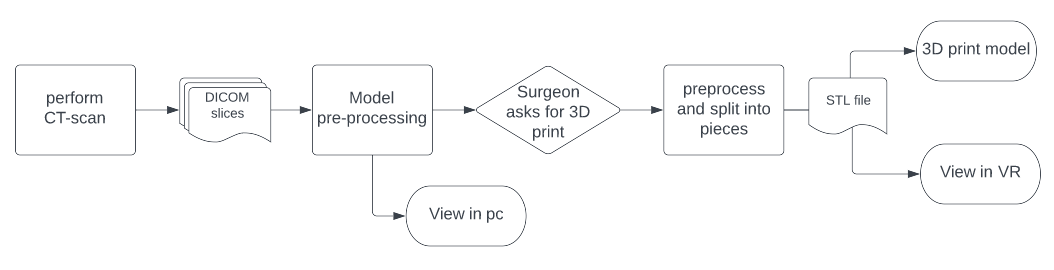
\includegraphics[width=1.2\textwidth]{images/arbeidsflyt.png}}%
	\hfill
  \caption{Workflow of how medical imaging is used}
  \label{arbeidsflyt}
  \small
\end{figure}

%workflow printing
When deemed necessary by the surgeon, a 3D printed model of the fracture is created. The 3D print requires a previous three-dimensional scan such as a CT. The model can improve the surgeon's understanding of the fracture, and allow the surgeon to adjust and practice with implants. The medical imaging and 3D printing is done by radiologists at the hospital.
A simplified typical workflow is shown in figure~\ref{arbeidsflyt}. This also shows a suggestion on how VR could be used in this process.

This project was based on elective surgery planning in a complicated fracture.

\subsection{Orthopedic methods}

Fracture treatment in orthopedics can be divided into several methods outlined in Textbook of Orthopedics~\cite{ebnezar_textbook_2016}.
Nonoperative methods include straps, slings or casts.
Nonoperative methods have no infection risk or surgical risk, but can result in bone not healing properly in complex fractures.

%internal fixation
Operative methods are used for anatomic reduction. Reduction is how bones are set in close proximity after a fracture, and is important for proper healing~\cite{verywell_health_fracture_nodate}.
When surgery is decided, the fracture is typically fixed internally by implants.
Internal Fixation means to internally set and stabilize bones~\cite{ebnezar_textbook_2016}.
Implants include screws, nails, and plates made from steel, titanium, or plastics.
Treatment of fractures by external fixation is also possible. External fixation means a metallic frame is connected to the bone with pins.

\subsection{Radiology}
Radiology is the use of medical imaging to diagnose and treat disease. A radiologist is a doctor interpreting images, while the technicans performing the imaging are radiographers~\cite{swiontkowski_manual_2013}.

The first used imaging tool was the X-Ray, discovered in 1895~\cite{hamblen_outline_2010}~\cite{suetens_fundamentals_2017}. As the energy in the radiation is absorbed at a different rate by tissue and bone mass, it is possible to create an image of the bone. The image is displayed as a projection from the X-ray angle. During the first half of the 20th century, additional techniques with several X-Rays allowed to isolate a slice of bone without over- and underlying tissue. Often X-ray from several angles is required to view the fracture without being obscured by other bone masses~\cite{ebnezar_textbook_2016}.

%CT scans
A big leap in medical imaging was the CT scan (computed tomography)~\cite{bradley_history_2008}.
CT scans (Computed Tomography) were invented during the 1970s. During a CT scan, an X-ray tube is rotated around the tissue, scanning from all angles while detecting the absorption/reflection of the tissue. CT scans overcome the two-dimensional X-ray limits and create detailed image data that can be visualized in any plane without superimposing the image with tissue above and below the selected layer~\cite{hamblen_outline_2010}. The detail of a CT scan depends on the hardware used, as well as the trade-off where higher resolution gives the patient higher radiation~\cite{bradley_history_2008}. The higher resolution is in complex cases preferred over X-ray to evaluate intra-articular fractures (crossing a joint) or locate smaller fractures~\cite{ebnezar_textbook_2016}.
CT scans can eliminate the need for repeated imaging in the case of a trauma patient~\cite{swiontkowski_manual_2013}.
MRI (Magnetic Resonance Imaging) was also developed during the 70s. It uses a strong magnetic field and radio signal frequencies to scan. MRI has comparable accuracy to CT but can also view soft tissue. MRI also avoids radiation~\cite{swiontkowski_manual_2013}.


The imaging used for testing in this report is from CT scans done by Radiological department of Haukeland University Hospital.

\subsection{Visualisation of medical imaging}


The output of both CT and MRI scans is a three-dimensional scan. The output is typically represented as slices, where a slice is a 2D picture repeating along an angle. The pixel at coordinate \emph{(x, y)} at slice number \emph{z} represent the absorption at the point \emph{(x, y, z)}~\cite{chougule_conversions_2013}.
Each pixel in a slice represents a voxel in a volume, and all the slices combined make up volumetric data or a three-dimensional point cloud~\cite{chougule_conversions_2013}.
The slice thickness of a slice can be below 1 mm, giving a high-resolution scan where a single point is less than one cubic millimeter~\cite{hamblen_outline_2010}. Figure \ref{dicom} shows the workflow of converting from slices to voxels and further to a mesh model.

\begin{figure}[h!]
    \centering
  \makebox[\textwidth][c]{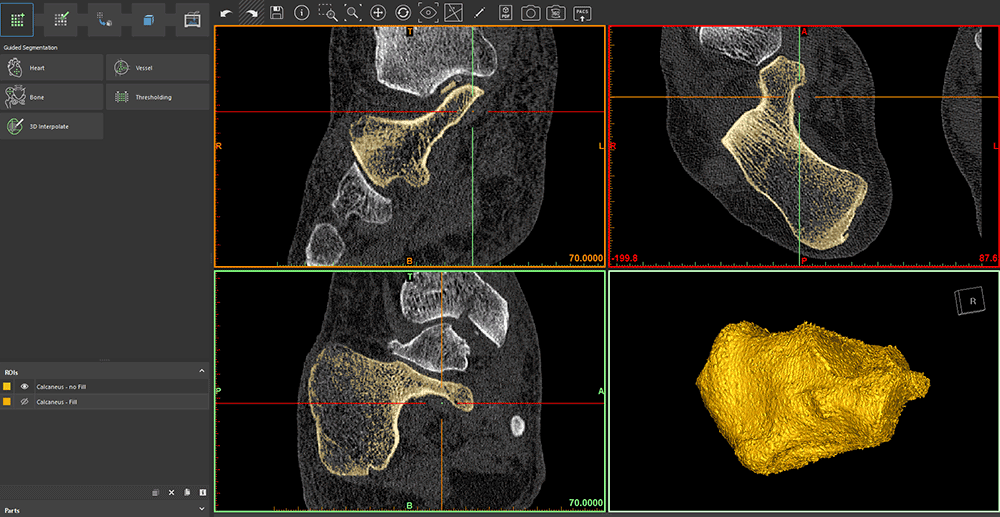
\includegraphics[width=0.8\textwidth]{images/materialise.png}}%
	\hfill
	\caption{Screenshot of Materialise application \cite{materialise_medical_nodate}}
 \label{mat}
\end{figure}

When rendering a 2D image, the volume must be projected to two-dimensional space. The values in a single slice can be used to view the intersection at a specific slice number. A line of values along all the slices can be used to view the intersection at another plane.
All slices can be combined to show either the average or the maximum intensity~\cite{fishman_volume_2006}.
The values are converted to greyscale by mapping ranges of values to greyscale pixels. This mapping function determines the brightness and contrast of the final image.

A specific algorithm is needed to render the scan as a 3D surface mesh. Rendering the model includes preprocessing the volume and classification to determine the type of tissue based on voxel value. A simple approach is thresholding, a binary classification where a polygon is created on any volume point that matches the threshold value. A different threshold can be selected to visualize tissue with different densities, typically bone~\cite{fishman_volume_2006}.

Figure \ref{mat} shows the application Materialise used at Haukland University Hospital. Both CT slices from different angles and a rendered model is shown side by side.

\begin{figure}[h!]
    \centering
  \makebox[\textwidth][c]{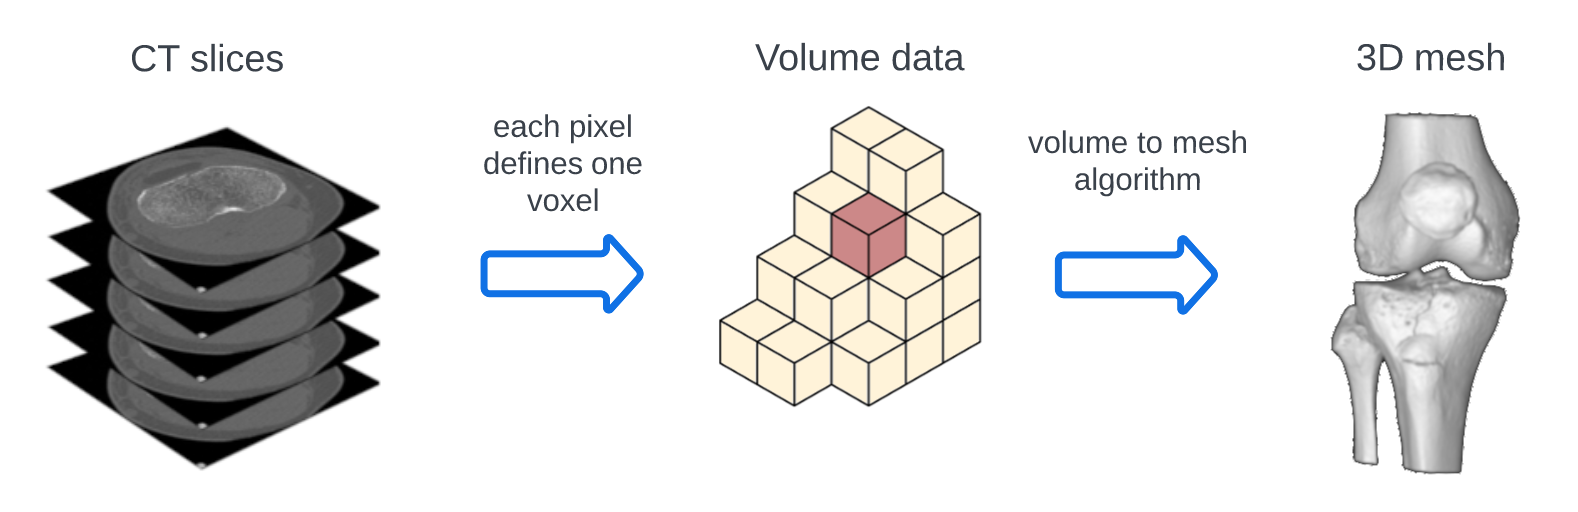
\includegraphics[width=1.2\textwidth]{images/slices.png}}%
	\hfill
  \caption{DICOM data conversion to a polygon mesh}
  \label{dicom}
\end{figure}

\subsubsection{Data formats}

The output of most medical imaging is standardized with the Digital Imaging and Communications in Medicine (DICOM) format~\cite{noauthor_dicom_nodate}. The DICOM format includes metadata and pixel data. CT scans are saved as several files, where each file represents one slice in the scan.

%obj and stl
If the data is represented as a 3D mesh, several formats can be used. The Wavefront Object file format (OBJ)~\cite{obj_wavefront_nodate} is a standard format for objects defined by polygons and surfaces. 3D mesh formats such as OBJ differs from DICOM by not storing volume data. Any density data is deleted when converting from DICOM to OBJ.
Another mesh format is the Stereo lithography file (STL)~\cite{noauthor_stl_2019}. The STL standard is created specifically for 3D printing. STL includes polygon info similar to OBJ files.

\subsubsection{ 3D printing }

An alternative to digital representation is to print the model with a 3D printer, illustrated in figure \ref{3dprint}. A 3D model can help increase accuracy when performing a procedure~\cite{shahrubudin_overview_2019}, especially in complex fractures~\cite{chen_efficacy_2019}. 
3D printing has many advantages, such as the surgeon physically holding the model, measuring the model, trying out equipment, and practicing with the model.

The most significant disadvantage to 3D printing is that the printing process can take more than 24 hours, depending on model size, materials, and printer. The waiting time is, in some cases, too long. 
Another drawback is not having any digital tools such as transparency control, displaying cross-sections, or being able to alter the model after it is printed. 
A physical plastic model also needs support structures that can lead to an inaccurate representation of the fracture or get in the way of viewing the model. The support structure issue is especially obvious in a fracture with many small bone fragments. A similar problem is not being able to print any fractures on the inside of volumes.

\begin{figure}[h!]
    \centering
  \makebox[\textwidth][c]{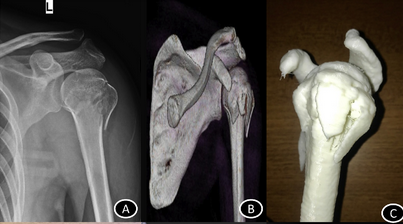
\includegraphics[width=0.8\textwidth]{images/ctToPrint.png}}%
	\hfill
  \caption{Humeral (upper arm) fracture}
  \label{3dprint}
  \small
    A fracture from initial scan to finished print. (A) preoperative X-ray; (B) 3D model; (C) 3D printed model.
\end{figure}

%cost of 3D printing
The cost of a 3D printer and material depends on printer type and size requirements but is typically low. Extrusion-based plastic printers are commercially available at as low as 200 USD/ 1800 NOK, with very cheap materials. The cost of 3D printing in industry or medicine comes from personnel, training, and time usage~\cite{shahrubudin_overview_2019}.

\section{Extended Reality}

% TODO: bilde av ar og vr???

Extended Reality (XR) \enquote{is devices capable of overlaying digital information onto the physical world or incorporating aspects of the physical world into virtual scenes}~\cite{andrews_extended_2019}.
XR is typically split into Virtual Reality (VR) and Augmented Reality (AR).
Virtual Reality is the use of VR technology to sense the user's state and actions and augment sensory feedback to immerse the user in a 3D virtual environment~\cite{mihelj_virtual_2014}.

The virtual reality system works by tricking the senses by displaying computer-generated stimuli that replace stimuli from the real world. 
The user typically perceives the virtual environment through a Head-mounted Display (HMD), sound, and haptic feedback (vibration).
The virtual environment is the computer-generated objects that the user interacts with. The virtual environment will often mimic properties in the real world, such as shape, color, or functionality.

With more specialized hardware, additional stimuli such as temperature, smell, and more are possible~\cite{noauthor_feelreal_nodate}.
To make the virtual environment seem real, it must respond to the user's actions. Current commercial Virtual Reality headsets track the user's head and hands and allow for button inputs~\cite{noauthor_oculus_nodate}. Modern HMDs use 6 Degrees of Freedom (DOF), which means the user is tracked in three-dimensional position and rotation~\cite{lang_introduction_2013}. The tracking is used by the VR application to simulate walking, picking up objects, and more.

\subsection{Augmented and Mixed Reality}
Augmented Reality and Mixed Reality (MR) is an addition to VR where the real world is viewed together with the digital environment~\cite{hackett_three-dimensional_2016}. Several definitions exists, according to Intel~\cite{intel_virtual_nodate} AR is a digital overlay onto the real world while MR means interacting with both digital and real elements.
For simplicity this thesis will use the term Augmented Reality to describe devices showing both a virtual and a real environment.

AR comes in different variants; some mobile apps use the camera to create an augmented environment shown in 2D. More expensive AR HMDs work similarly to VR HMDs, except for the transparent viewing glass. Mixed Reality devices primarily exists as expensive HMDs, such as the Hololens~\cite{hololens_microsoft_nodate}.
AR HMDs are used in medical, industrial, and military devices to show critical information while users operate devices or perform a job in real life. Examples of this are a surgeon viewing medical information during a surgery or a pilot viewing a Heads Up Display while flying~\cite{mihelj_virtual_2014}~\cite{mertz_virtual_2019}.
AR has some uses not relevant to VR because it does not completely disconnect the user from the real world, but has some disadvantages such as reduced field of view compared to VR, poor visibility in bright light~\cite{hackett_three-dimensional_2016} and drastically higher cost~\cite{medical_holodeck_medicalholodeck_nodate}.

\subsection{Professional usage of XR}
While becoming more popular in mainstream entertainment, XR has been used in professional environments for many years.
An advantage of XR compared to mouse and keyboard devices is touch-free interfaces with hand tracking, making it better for a sterile environment~\cite{andrews_extended_2019}.

VR has been developed by the US Airforce since the 1980s for pilot interfaces~\cite{mertz_virtual_2019}. VR and AR are often used in the medical field for training or education because the actual situation would be unpractical or dangerous~\cite{freina_immersive_2015}.
VR is used in cardiology and neurology for monitoring and is emerging in other medical fields such as rehabilitation and training~\cite{javaid_virtual_2020}.
VR can also be used in medical fields for equipment training, like the radiologist training program in figure~\ref{training}. This allows for training with equipment that are expensive, currently unavailable or unpractical to train with.

\begin{figure}[h!]
    \centering
  \makebox[\textwidth][c]{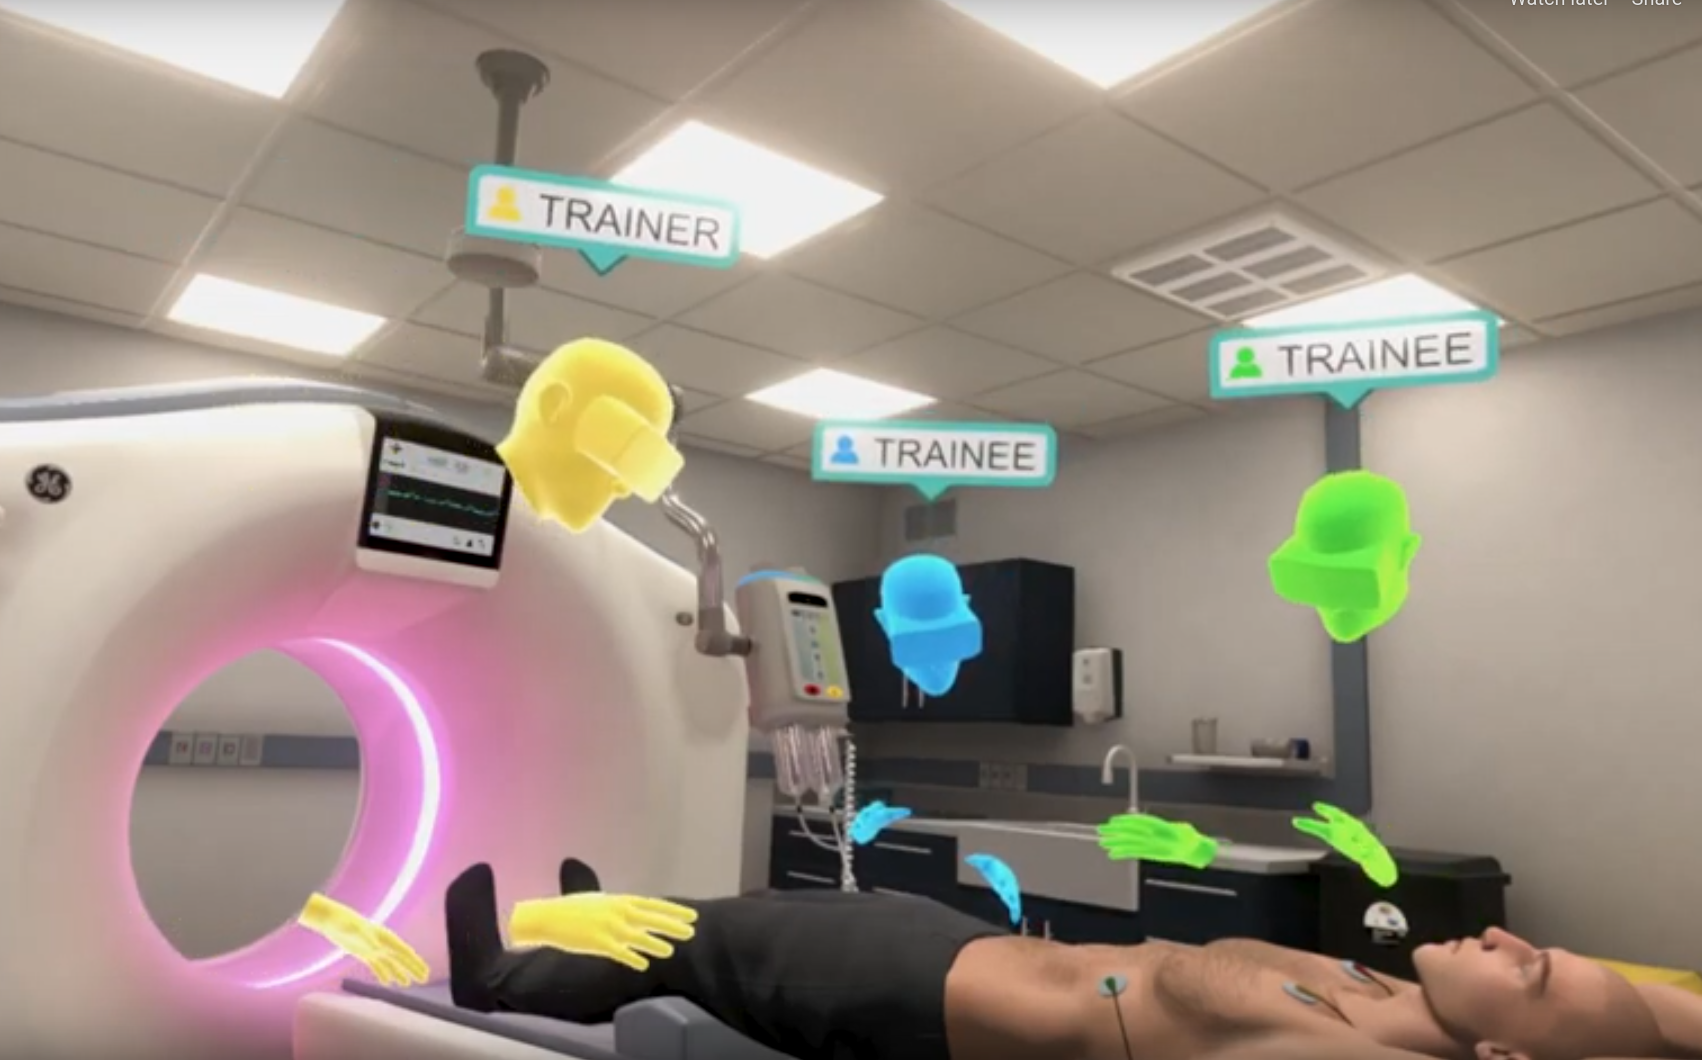
\includegraphics[width=0.8\textwidth]{images/training.png}}%
	\hfill
  \caption{Radiologist training in VR}
  \label{training}
  \small
Multiple users in a virtual training environment practicing using a CT scanner.

Image from website HealthySimulation~\cite{noauthor_how_2020}
\end{figure}

% TODO: mer om medisin?

\subsection{Advantages and disadvantages}
A disadvantage with wearing an HMD is fatigue, both physical fatigue caused by the weight or eye fatigue and motion sickness~\cite{merhi_motion_2007}.
Image imperfections cause eye fatigue in the HMD~\cite{kooi_visual_2004}, and motion sickness is caused by sensory conflict.
According to a study on motion sickness factors, 59 \% of the subjects experienced motion sickness after 14 minutes on average. The remaining subjects did not experience any illness~\cite{kooi_visual_2004}. However, Motion sickness can be mitigated in several ways described later.

A use-case of XR is simulating a subject physically out of reach, such as a planet in space or the inside of a patient's knee. For physically impaired users, this advantage is even more relevant.
XR can also simulate situations that would otherwise be dangerous, for example, an untrained surgeon performing surgery alone.
Another advantage is that VR is more immersive than other mediums. The immersion makes the user feel more stress or fear and makes it feasible to prepare personnel for stressful situations, such as the police.
The added immersion also makes teaching or training more motivating for students~\cite{freina_immersive_2015} and improves learning outcomes~\cite{cynthia_l_foronda_virtual_nodate}.

\subsection{Designing for VR}
VR is relatively new in mainstream media, and as such, there are few agreed-upon standards for designing the User Experience (UX).
Common VR tips from game designers~\cite{vrdesign_best_nodate}~\cite{vrdesignadobe_virtual_nodate} are immersing the user in a enviroment with real life interactions instead of just text. Other tips include keeping the user comfortable by keeping the user in control of movement, avoiding bright colors and placing objects at a appropriate height.

Some practical measures to counter motion sickness and fatigue are reducing Field of View (FOV), varying latency between user input and display update, flickering, moving content in the virtual environment, and using several stimuli (audio, haptic feedback)~\cite{chang_virtual_2020}. 
Some of these are hardware-dependent and not relevant for this project, so moving content is the most relevant measure in this project.

\subsection{Game Engine}
A game engine is a framework specifically used for developing games~\cite{gameengine_what_nodate}. Several third party game engines are available, the most popular being Unity and Unreal Engine.
Using a game engine speeds up the development as it includes systems needed, like rendering, animations, and physics.

%why unity
The Unity game engine~\cite{technologies_unity_nodate} was used for developing the application. Unity is widely used for game development~\cite{doucet_game_2021} and is well documented online with a lot of community-supported plugins. The author also had previous experience with Unity development.
Unity has good support for different VR and XR platforms~\cite{technologies_unity_nodate-3} including the OpenXR standard widely used by commercial VR headsets~\cite{noauthor_openxr_2016}. OpenXR allows creating VR games with Unity handling most VR logic.

Part of the Unity VR support is the XR interaction Toolkit (XRTK)~\cite{noauthor_xr_nodate}. It is a high-level framework for using XR interactions with Unity events. The toolkit also includes components for selecting/grabbing, haptic feedback, and button interaction.

To develop for several XR platforms, the different controllers have a mutual interface for setting keybindings, called an XR controller. Almost all commercial VR controllers support an index finger trigger, a joystick/trackpad with 2D directional input, a grip button, and at least one extra button~\cite{technologies_unity_nodate}.

\subsubsection{Entity Component System}
Development in Unity is based around the Entity Component System~\cite{entitycomponent_entities_nodate}. An entity is every object populating the game. The base class for all entities is the GameObject. Every model, player and menu is a GameObject.

Components attaches to one or more Entities to define the behaviour. Entities can have several components. Components can provide game logic, movement, user input and much more. Components are scripted in C\# and the .NET framework.




\chapter{Design and Implementation}\label{Design and Implementation}
The author developed the application in 6 months. The author had no medical experience and dependent on support by staff at Helse vest with guidance on medical projects and expertise in orthopedics, medical imaging and VR development.

\section{Demonstration}\label{demonstration}
gameplay

\section{Design methods}

\subsection{Research Method}
The research question was answered by evaluating the VR application regarding the research questions. A mixed testing method was used to evaluate the application.

The most significant part of the study was developing the application that fills the need for viewing CT data. This was accomplished by uncovering user needs with interviews and testing the application on users. When the application met minimum specifications, an evaluation was performed.

The evaluation at the end of the project aims to answer both research questions. The evaluation was done in the following way:
The project participants use the application on their own in a relevant scenario until they feel they have performed the task.
The users respond to a System Usability Scale form and a semi-structured interview. The questions are specific to the research questions and either a planning or an educational use case.

The responses are gathered and used to discuss the research questions.

\subsection{Iterative Development}

\begin{figure}[h!]
    \centering
  \makebox[\textwidth][c]{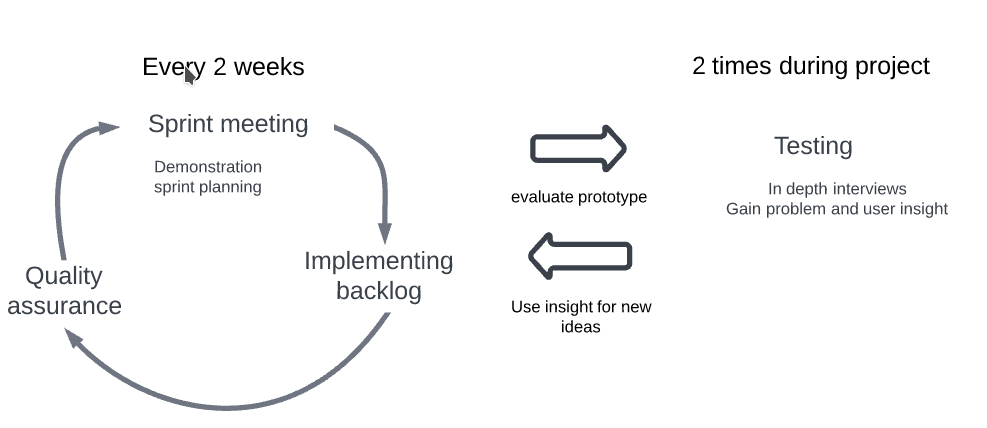
\includegraphics[width=1.3\textwidth]{images/agile.png}}%
	\hfill
  \caption{Development method}
  \label{agile}
  \small
  weekly iterations illustrated on the left, and user testing on the right.
\end{figure}

The application is developed using iterative development and elements from Design Thinking~\cite{razzouk_what_2012}.

% Why iterative
Iterative development was used to cooperate effectively with the team and increase the development speed. The team had regular meetings, and this fits well with the iterative cycles (figure \ref{agile}). The cycles facilitated frequent feedback from the domain experts. The feedback could then be implemented and tested at the next meeting.

TODO: bilde av early prototype?

% cycle structure
The team had regular biweekly meetings with a demonstration and next iteration planning. The meeting was a valuable way of sharing interdisciplinary information and getting feedback from domain experts. Scrum elements such as Sprint retrospective and daily scrum were not relevant as only one person worked full time on the project.
After the demonstration, the backlog was updated with tasks prioritized by value. The value is determined by the time needed to implement compared to how important the functionality is to the product owner. The top tasks that fit within two weeks are added to the backlog, and the remaining are stored in the product backlog and considered for the next cycle.
During the next two weeks, as many tasks as possible were implemented and demonstrated in the next meeting.

% conclusion
The frequent meeting demonstrations worked really well with VR development, as the different features are hard to understand without trying the application. Fast iterations are essential to cooperate efficiently when the product owner or test users have a limited understanding of the technology.

% design thinking
Design thinking elements was used because both the medical domain and user needs were challenging to understand. Specifically the empathise, define and ideate stages was used. Frequent prototyping would be too time consuming too be relevant. Design Thinking helps to understand an unfamiliar domain and what the needs of the users are.
The application demos served as smaller user testing sessions. The medical personnel in the team would try out the application and any new features and give feedback and ideas during testing. User testing would often lead to new ideas. Optimally the test subjects should have been personnel outside the project without any bias, but busy schedules and COVID restrictions limited this.

% testing
A more in-depth user testing was done twice in the project. This included testing the application with orthopedic surgeons to gain more insight into user experience and user needs. Optimally this would be done frequently at the end of iterations, but the test users were unavailable. The tests are described in detail in a later chapter.

\section{Project overview}\label{CodeStructure}

\section{Design}

% \subsection{Design goals}

The final product is a VR viewer for viewing STL files and DICOM data. A VR solution was selected for faster development and better hardware availability than AR, while the AR advantages were not relevant for the planning phase.
The solution uses the STL files and DICOM data already produced at the hospital and requires no extra data other than what is used for 3D printing.

The primary goal for the UX design is ease of use for non-technical users, as current VR solutions at Haukland University Hospital are cumbersome programs.
A secondary goal is to make users understand the anatomy well and facilitate for surgery planning.

\subsection{Hardware}
The VR devices used for this development and testing was the Oculus Quest 1 and Quest 2~\cite{noauthor_oculus_nodate}. The hardware was selected out of availability reasons and the practicality of having a standalone device.
The Quest 1 and 2 are very popular consumer standalone VR headsets. When in standalone mode, the headset uses integrated graphics and is battery powered. The standalone mode performance is far inferior to a headset connected to a powerful computer, as can be seen in figure~\ref{comp} the Quest struggles with dense geometry, textures and post-processing effects.
There are other headsets with better displays and motion tracking, but the Quest devices are sufficient.

\begin{figure}[h!]
    \centering

  \makebox[\textwidth][c]{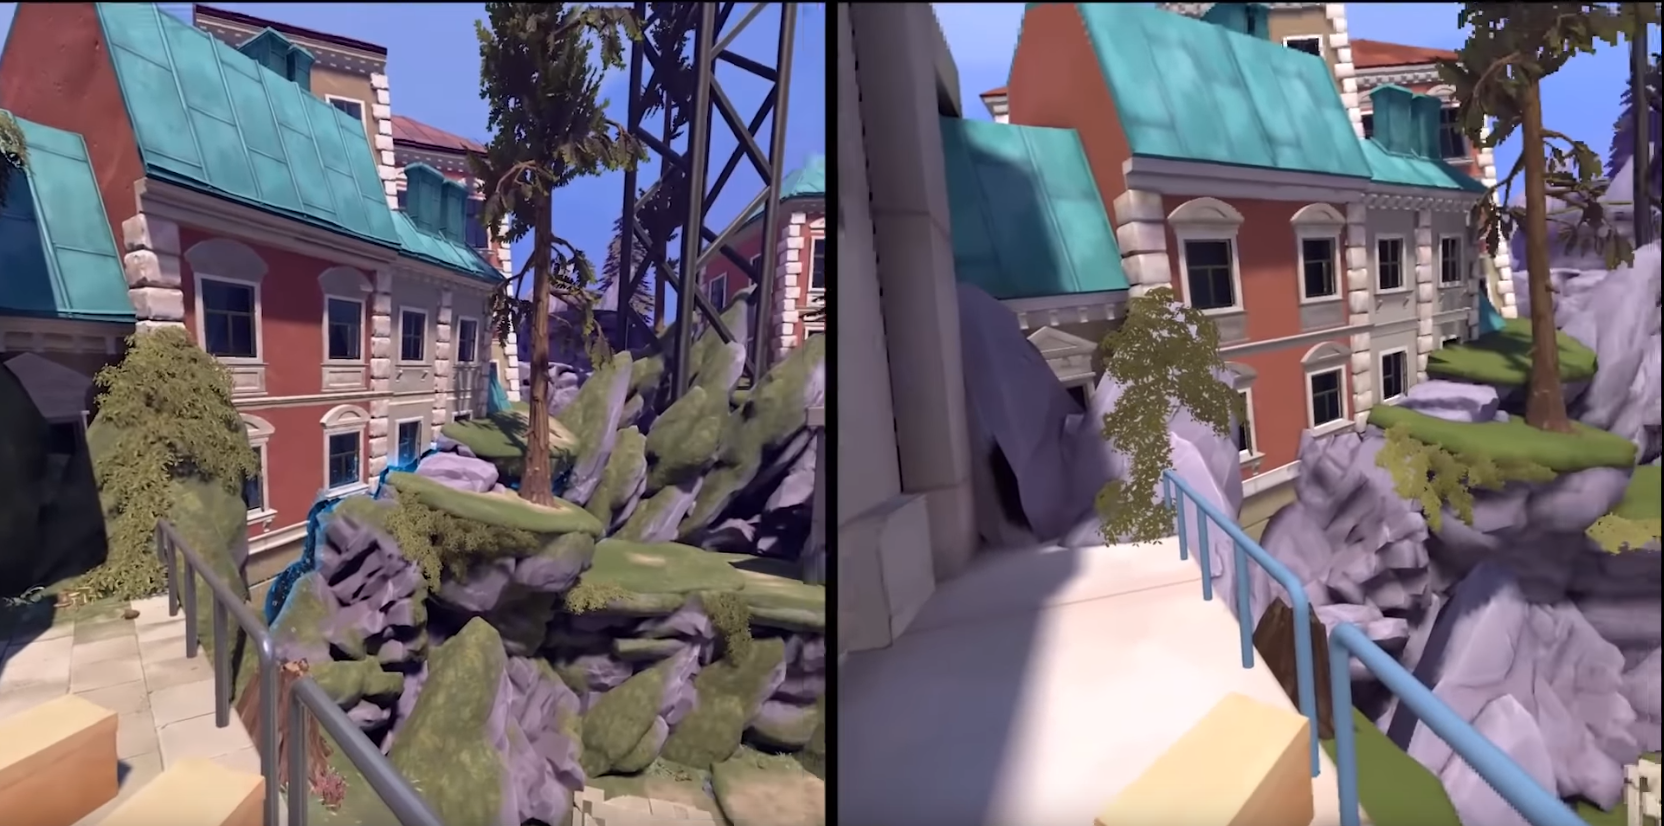
\includegraphics[width=1.2\textwidth]{images/comparison.png}}%
	\hfill
	\caption{The video game \emph{Apex Legends} running on a desktop computer compared to Quest 1 in standalone mode~\cite{tyriel_wood_-_vr_tech_oculus_2019}.}\label{comp}
  \small

\end{figure}
%how it worked
Testing in standalone mode at different locations was very convenient, but it had a drawback as the project needed to be tailored to run on a low performance android device. This led to problems with both high resolution data and different bugs related to the android build.

\subsection{VR interface}

% TODO: Overview image

To make the VR interface easy to use, the focus was primarily on familiarity with current tools and a simple design.
I used MicroDICOM~\cite{noauthor_dicom_nodate-1} as a reference for a familiar tool.
Familiarity with current tools means taking interactions from programs such as CT viewers and adopting the same interactions to VR to make it recognizable and consistent to the user. An example of this is navigating a menu in VR the same way one would navigate a menu with a pc mouse.
 All unnecessary interactions and information is removed to allow new users with little VR experience to start using the program quickly. The goal is to make the experience less overwhelming and lower the skill required to use the viewer effectively.

\subsubsection{Architecture}
The architecture of the Unity application is based around a singleton 'GameController' module. The GameController manages important states and contains references to the other modules, shown in figure~\ref{structure}. The modules have different responsibilities like multiplayer or menu interaction and communicates through the GameController. This solution is easy to extend and prevents a lot of cross-references between components.
%gameobjects
A module typically consists of a GameObject with the same name, and one or more components attached to the GameObject. In some cases the GameObject has several GameObjects as children.
As an example the Model Container has a child for every part of the model. This is indicated by one to many relationships in the figure~\ref{structure}.

The components related to the model have several instances and are drawn as one-to-many relations in the figure. This allows to swap between models while keeping info on positions and implants.

\begin{figure}[h!]
    \centering

  \makebox[\textwidth][c]{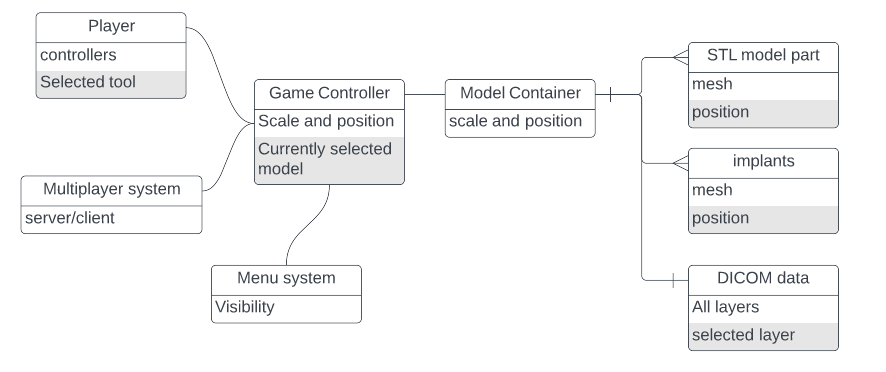
\includegraphics[width=1.3\textwidth]{images/structure.png}}%
	% \subfloat[][]{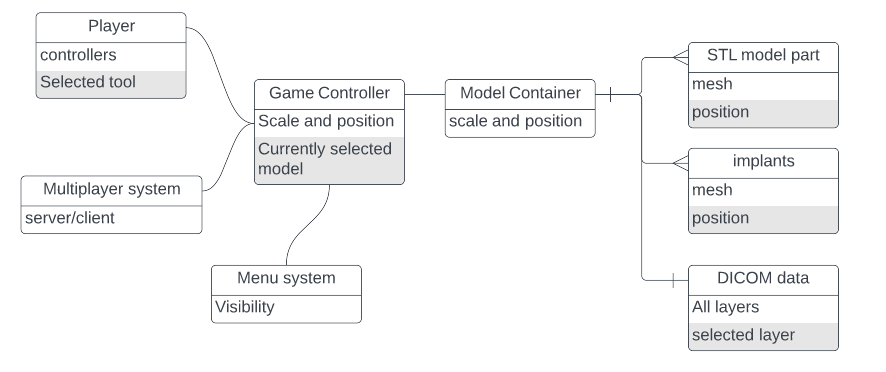
\includegraphics[height=160pt]{images/structure.png}}
	\hfill
  \caption{Unity project modules}\label{structure}
  \small

\end{figure}

\subsubsection{Learning process}
A video game style tutorial was considered, where the user would go through tasks with hints or descriptions of the features in the application. However, this was not implemented as early testing revealed both experienced and inexperienced users were learning the controls quickly.

As an alternative to the tutorial, a hint system is implemented. Every button has a description displayed as text above the button to remind the user of the keybindings as in figure~\ref{hints}. An image can optionally be displayed, showing the user the keybindings. The hints were implemented as users repeatedly forgot button controls in testing.

\begin{figure}[h!]
    \centering
	\subfloat[][]{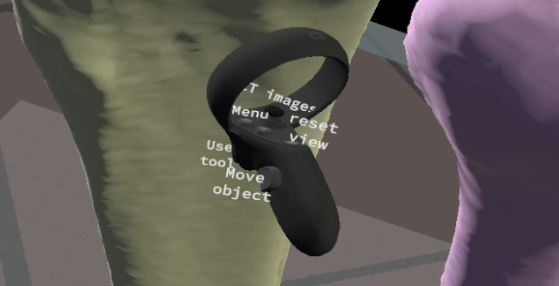
\includegraphics[height=160pt]{images/buttonhintscrop.png}}
	\hfill
  \caption{Controller hints}\label{hints}
  \small
\end{figure}

\subsubsection{Grab interaction}

One of the core features in the user interface is moving fracture parts to inspect or rearrange them. Rearranging is important for fixation planning, and inspecting from different angles is useful for anatomy understanding.
The grabbing action should mimic how users grab objects in real life to make the action easy to use. When the user places a hand close to a model part, the color is tinted to highlight the chosen part. When the grab button is pressed, the highlighted model part is picked up, and a short audio clip is played. The model part will then follow the user's hand as long as the button is held.

\begin{figure}[h!]
    \centering
	\subfloat[][]{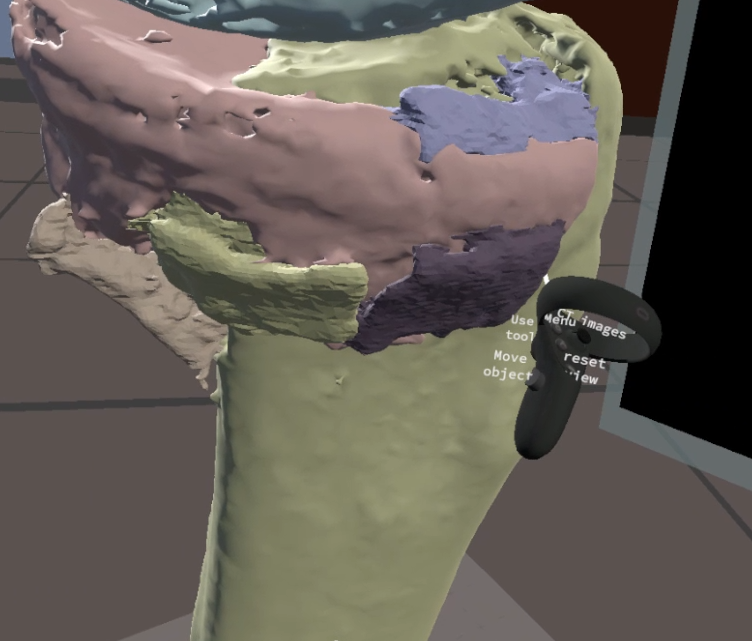
\includegraphics[height=199pt]{images/grabinteraction.png}}
	\hfill
  \caption{Grabbing an object}\label{grabbing}
  \small
  Notice how the model part close to the controller is focused with a darker color.
\end{figure}

One issue is whether the user wants to move either the entire model or move a part of the model when grabbing. Including both could introduce mode issues~\cite{experience_modes_nodate}, so the grab can only have one use.
It was decided that the grab interaction always picks up a model part. A joystick input moves the entire model, which is less precise than grabbing.

The grab functionality is implemented using Unity's built-in $Interactable$ system for XR~\cite{noauthor_xr_nodate} development. This allows to set up grabbing, throwing, and more.
In the $Interactable$ system the grab moves the center of the object to the user's hand when grabbed. This built-in grab action is cumbersome when precisely adjusting larger objects, as moving an object a small distance requires repositioning it from wherever the center of the object is.
To solve this, the interactable script is modified to keep the current position when grabbed and then follow the relative motion of the hand.

To allow for grabbing small objects or objects that are partly overlapping, the closest object is always selected.
The default Unity XR behavior is selecting a new object in every frame, and this would lead to the user grabbing several objects simultaneously. To solve this, any interactable is highlighted when the users hand is within the collision box, as in figure \ref{grabbing}. It stays highlighted until the hand is outside of the collision box. The grab action is only allowed to select the hovered object, until the grab is released.

Using Occulus hand tracking~\cite{noauthor_set_nodate} could be beneficial, but is currently not recommended for high degrees of precision. Future versions of hand tracking or Hololens hand tracking could improve the interact experience in the future.


\begin{figure}[h!]
    \centering
  \makebox[\textwidth][c]{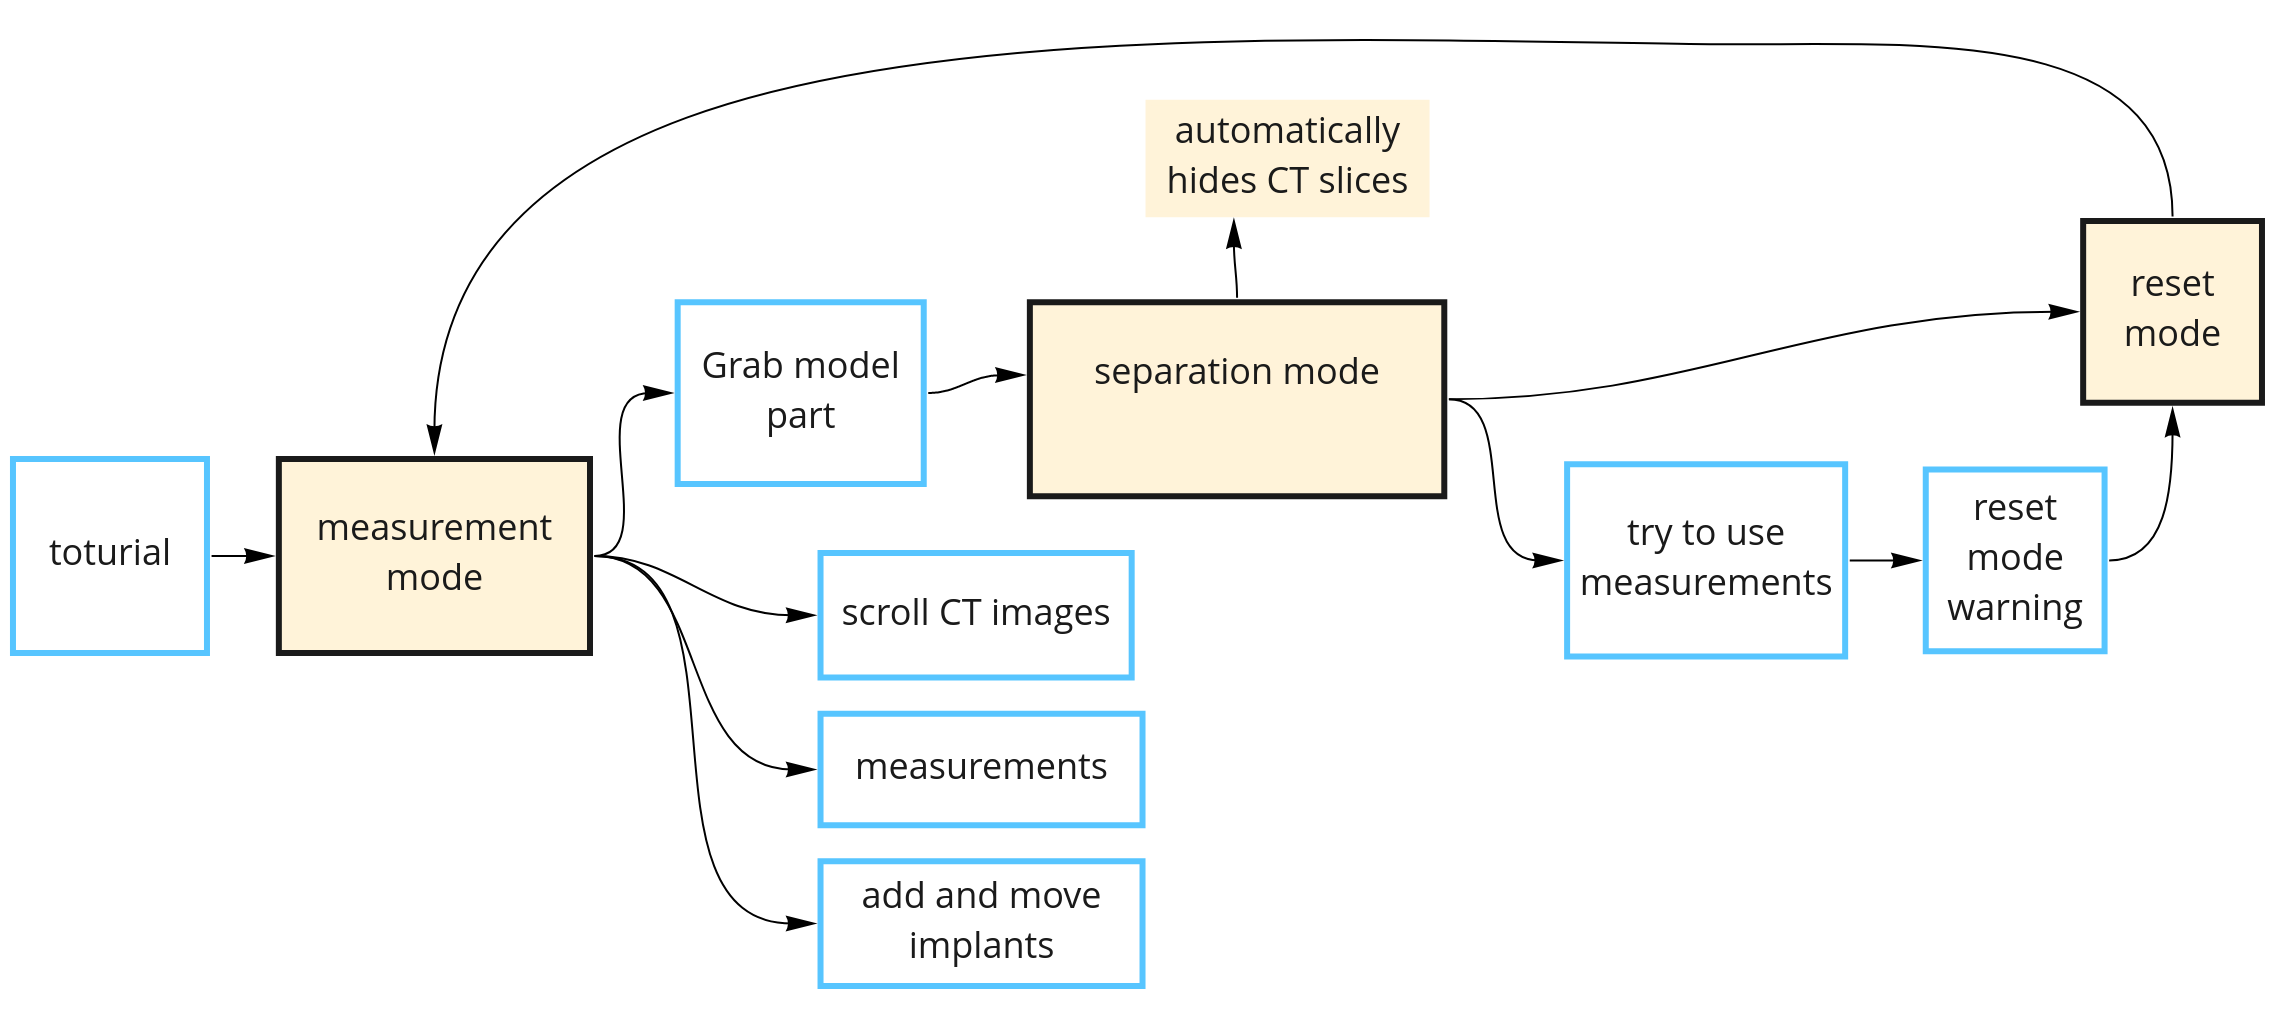
\includegraphics[width=1.1\textwidth]{images/flow.png}}%
	\hfill
	\caption{User flow}\label{flow}
  \small
  How the user changes moves between different states
\end{figure}

\subsubsection{Modal design}
The grabbing functionality introduces a problem: If the user moves a model part, the CT images will no longer be similar to the model displayed. Also, if the user is measuring the distance between two model parts, it gives an invalid result if the parts are moved.

The solution to this is a separation mode and a measurement mode. This is a modal design where the possible actions are dependent on the state of the application. The user can either move model parts around or view CT data and measurements. Moving any model part enters separation mode and reverting to the original position enters measurement mode. In separation mode, the CT images are hidden, and measurements are hidden. A large button appears to display the current mode, prompting the user to click the button to reset the model and once again view CT images and measurements.

\subsubsection{Keybindings}
Controller keybindings shown in figure \ref{controllers} was set to make the controllers intuitive and easy to use. This configuration seemed to work well in testing.

\begin{figure}[h!]
    \centering
	\subfloat[][]{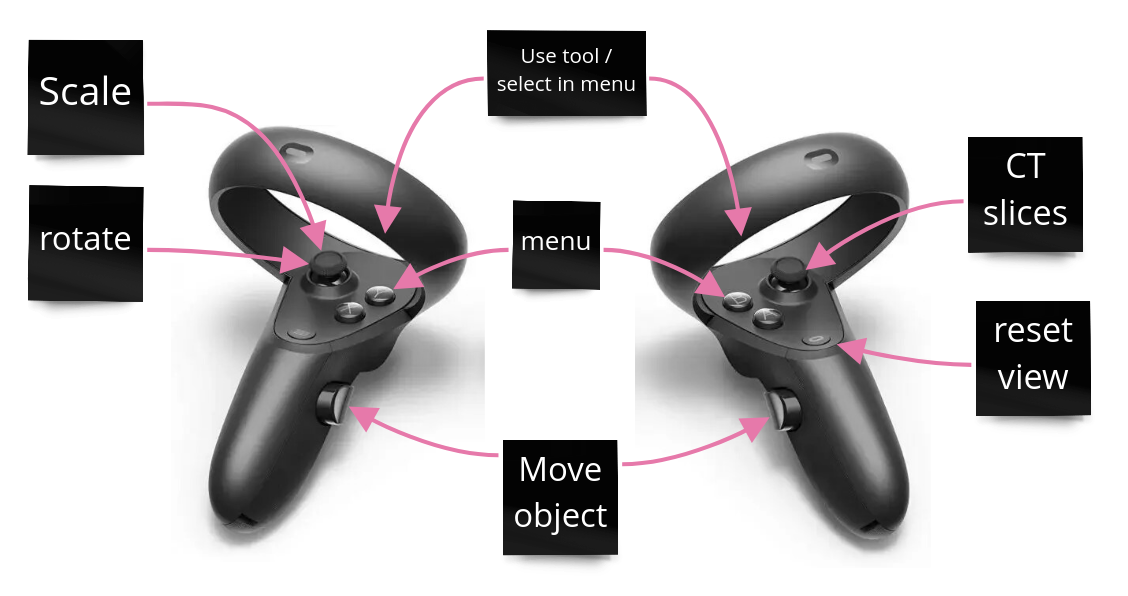
\includegraphics[height=180pt]{images/controllers.png}}
	\hfill
	\caption{Keybindings on Quest controllers}\label{controllers}
  \small
  This illustration is also used within the application.
\end{figure}

The most common operations are bound to trigger and grip button, which is easily reachable on most controllers. The controller trigger mimics a mouse click on a pc, and so it is used for clicking buttons and using selected tools. The grip button mimics a real-world grabbing gesture and is used for grabbing a model part.
The primary button is used for opening the menu.
For ease of use, the two controllers are mostly mirrored, except for the joystick. The right joystick is used for scrolling through CT slices, similar to how the scroll wheel is used in CT image viewers. The left joystick rotates and scales the entire model while keeping all the model parts correctly positioned.

The trigger button is also used for menu selection for consistency with other VR apps. This introduces conflicting keybindings with the $use\ tool$ button. This is solved by only performing one of the actions based on the context. If a menu is open or a button is hovered, a menu click is performed. Otherwise, $use\ tool$ is performed. This workaround simplifies the controls by using less buttons.

\subsubsection{Menu system}
A menu system is implemented to allow the user to navigate less common operations. The different operations are shown in~\ref{menu}.
When the menu button is pressed, the menu screen appears in front of the user. It is shown in world space, which means the text appears as a physical screen. The model is temporarily hidden to ensure the menu is always in the user's field of view. Placing content at the center of the screen avoids a typical VR UX problem where some information is not visible to the user.

\begin{figure}[h!]
    \centering
	\subfloat[][]{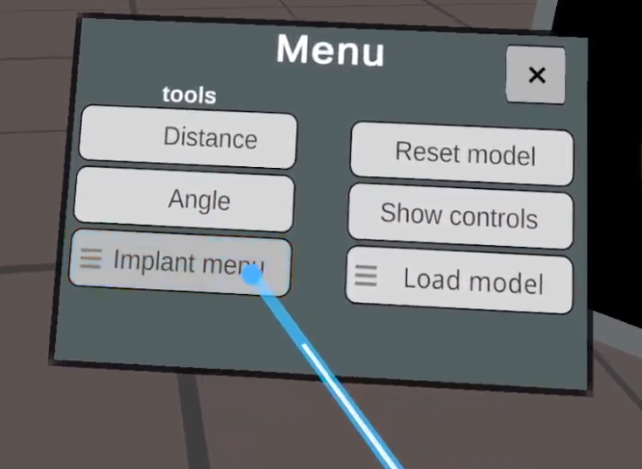
\includegraphics[height=180pt]{images/menu.png}}
	\hfill
	\caption{Menu screen}\label{menu}
  \small
  The main menu interface. The user is pointing at one of the buttons.
\end{figure}

The menu includes access to less frequent actions that do not require their own keybinding. The initial menu includes fast access to simple tools (e.g., measurement) and buttons to sub-menus. A hamburger menu icon suggests the button leads to a sub-menu.

The menu layout consists of one or more vertical lists of buttons. Several columns of lists are used to separate buttons into categories. To keep the menu simple and consistent, only buttons are used for interacting with the menu. The 'cross' button from pc programs is used for exiting the menu.
The sub-menus are implemented when multiple options are present. It is used for selecting an implant type or loading a new dataset.


\subsubsection{Measurements}
The most used functionality available in desktop CT viewers should also be available in the VR viewer. The needed tools are, according to early testing, measurement of distance and measurement of angles. Taking measurements allows surgeons to estimate sizes and plan what tools to use during a surgery.
Figure \ref{measure} shows a distance measurement.

The measure tools works by selecting a start and an end point. The angle measurement additionally requires a middle point.
After placing the first point, a preview of the measurement result is shown as a line to give feedback to the user of the current state.
Using the outline shader mentioned previously makes it possible to see the placed points even when obscured by the model, and the line between the points is always visible. This, combined with depth in VR makes it easy to understand where the points are placed and what the length and angle is.

\begin{figure}[h!]
    \centering
	\subfloat[][]{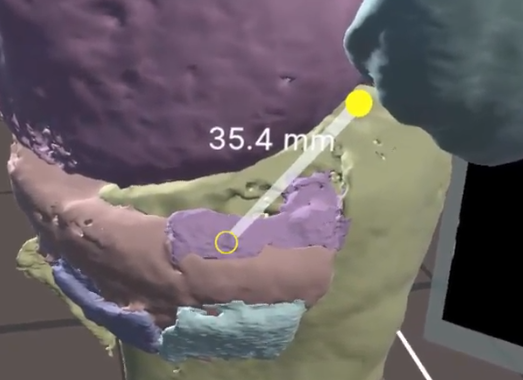
\includegraphics[height=190pt]{images/measure.png}}
	\hfill
	\caption{Distance measurement}\label{measure}
  \small
  The yellow hollow circle is inside the model with outline rendered on top. The filled circle is in front of the model. Distance in mm also drawn on top.
\end{figure}

\subsubsection{Audio}
Audio is mainly used for interaction feedback. If the user successfully picks up a model part, a sound is played to indicate the user is holding something. Audio is also used for feedback on the measurement tools. Audio in VR increases presence and investment and reduces distractions~\cite{kern_audio_2020}.

\subsubsection{Motion sickness}
The most relevant motion sickness factor for this project was the use of motion and static content. The only moving content is the fracture model, which only moves because of player input. The environment is designed like an office room and is always static. All menus and other objects are also static, with a few exceptions.
During multiplayer, the model may move caused by another player's input, which might cause some motion sickness if the model is viewed by the user. This could be solved by hiding the model when it moves, but it could interfere with the multiplayer experience if the model suddenly disappears.

\subsection{Multiplayer design}
The network discovery and session connection parts required for pairing two Quest devices over local networks or internet was not completed due to some network issues and lack of time. Multiplayer was not used in testing, but questions were still asked regarding its usefulness during interviews.

The goal of the multiplayer feature was to allow two or more surgeons to cooperate effectively. Having one surgeon using a VR headset and another using a screen is likely interfering because the surgeons are seeing different models. The multiplayer component allows the surgeons to use the same tools while seeing the same model, and should increase communication and cooperation.
Multiplayer should not make the application more difficult to use. All interactions should be similar to the usual experience, and cooperation should not require any extra steps, except connecting to the multiplayer server. Any important information should be available to all players, and irrelevant information (another player opening a menu) should not disturb users.

\begin{figure}[h!]
    \centering
	\subfloat[][]{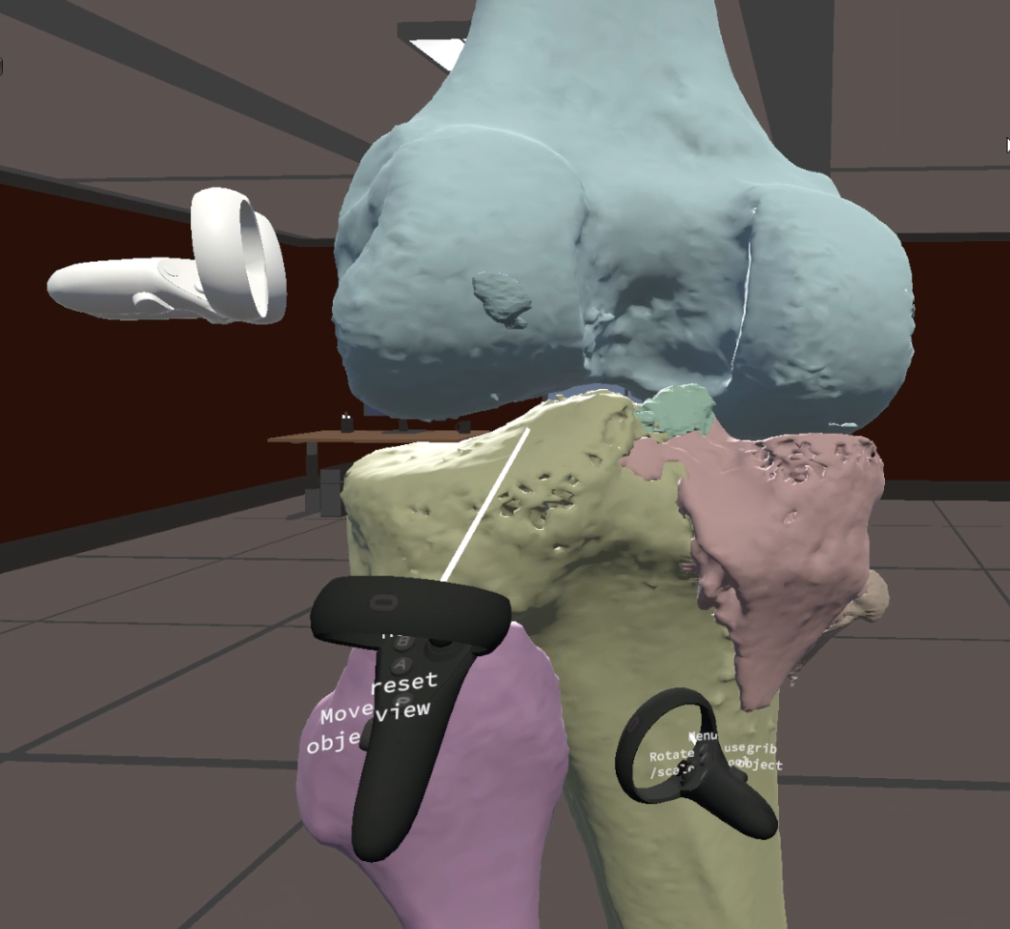
\includegraphics[height=220pt]{images/multiplayer.png}}
	\hfill
	\caption{Multiplayer}\label{multiplayer}
  \small
  Image showing a session with another user with white controllers.
\end{figure}

The multiplayer interface is a menu shown at startup. The user can select either to start a new session in which other users can join, or join an existing session. The sessions are hard-coded to always run on the same network port and have no authentication, as this would take too much development time and give no value. The server is also hosted by the user starting the session instead of a dedicated server, for easier development.

%how it works
All model parts are synchronized between players, so any models and movements is visible for all users. The position is continuously shared whenever a user is grabbing a model. As shown in figure \ref{multiplayer} other users' controllers are also visible in order to communicate and point at locations.


\subsubsection{Mirror}
The networking was built with Mirror, a downloadable Unity asset. Mirror is a high-level networking API built on deprecated Unity networking~\cite{noauthor_mirror_nodate}. Mirror has good support for creating a client/server pattern and classic video game related operations such as spawning in players at the start of the game and synchronizing objects across all clients.

\section{DICOM data visualisation}
I received several anonymized CT scan files from Helse Vest to use as input data. The CT scans are sent as DICOM packages, where the scan is stored as several files, each representing a slice.
The model is also split up into separate bone fragments by radiologists at Haukeland University Hospital. The files include 3D surface models as STL files, where each file contains one bone. The STL files allows to easily set up bone fragments as separate grabbable objects.


\subsection{Unity with custom file types}

To be able to read the DICOM files, the build produced by Unity needs access to the files. Unity has several built-in solutions to this.
The most common is the Resources functionality~\cite{resourcesload_unity_nodate} that builds the application and includes all files in a `Resources' folder. Android projects are built in the standard APK format and also require special file paths and using the built-in web request to read files. This is not well documented, especially for the Quest, so this method was scrapped.

The easiest way of referencing files is usually setting a reference in the unity editor, and the file will be included in the build. This works great with common files like images, but Unity does not allow custom file types without 'hacking' the Unity inspector and creating a custom file importer~\cite{scriptedimporters_unity_nodate}, that has lacking documentation. The solution to this is to rename all DICOM files to {name}.bytes. This makes Unity handle the files as 'TextAsset' text files~\cite{textassets_unity_nodate}. The files are then opened as text files and create a byte stream. The byte stream is then used for rendering with the DICOM library.

\subsection{Rendering CT images}

The user can view CT slices in 2D while simultaneously viewing the model as illustrated in figure \ref{ctscan}. This is done because of two reasons: to bridge the gap going from traditional 2D images to VR and retain the density data lost when converting to a mesh model.
An additional benefit is the use case of practicing interpreting CT images while viewing the corresponding model. The selected CT image is also shown as a transparent plane on the 3D model, to easily understand what the CT slice represents and further connect the images to the model.

\begin{figure}[h!]
    \centering
  \makebox[\textwidth][c]{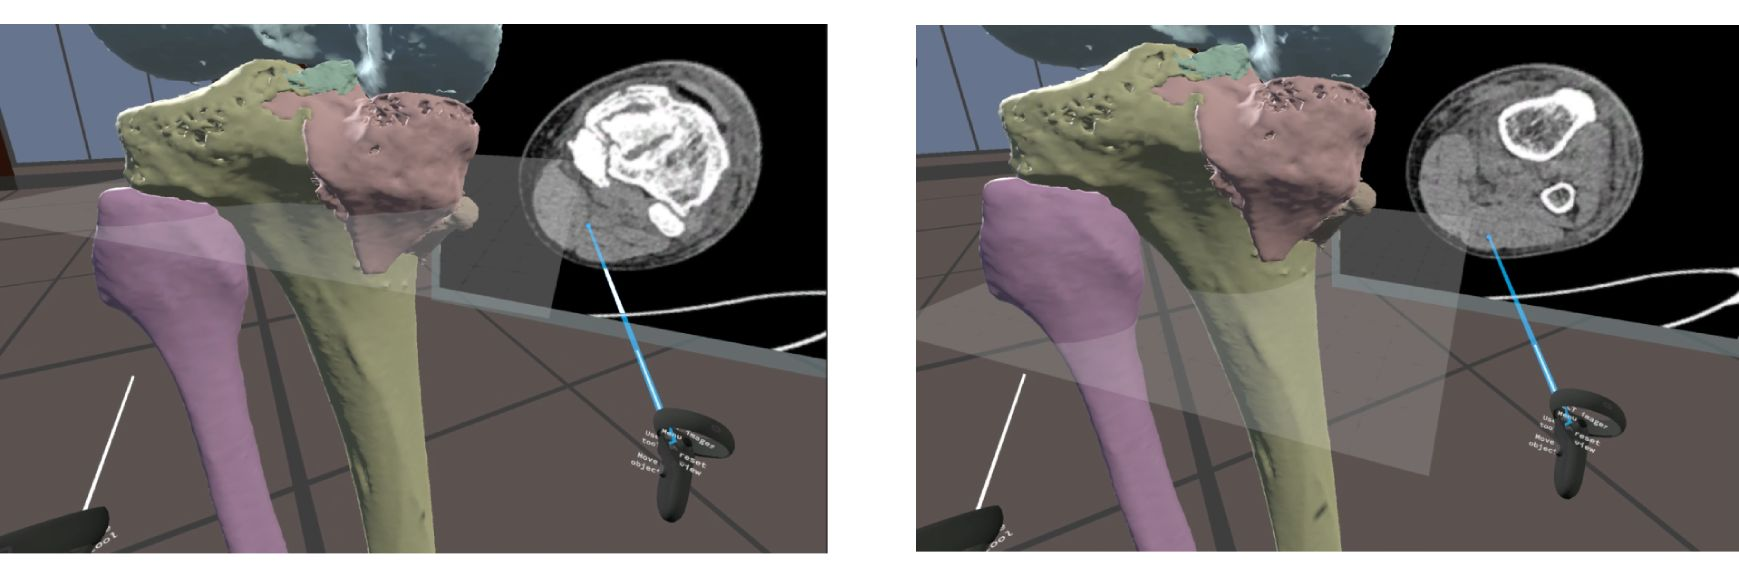
\includegraphics[width=1.3\textwidth]{images/ctscan.jpg}}%
	% \subfloat[][]{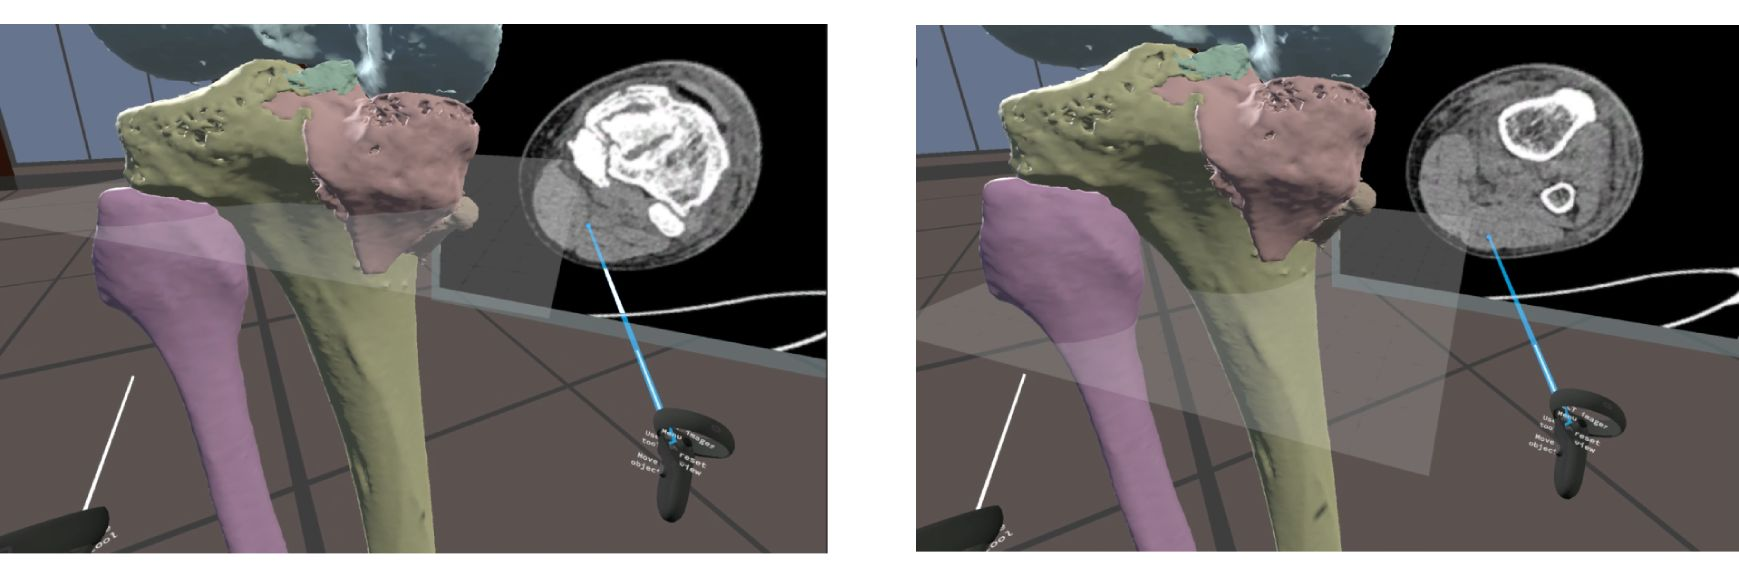
\includegraphics[height=120pt]{images/ctscan.jpg}}
	\hfill
	\caption{CT image}\label{ctscan}
  \small
 The user is moving the CT slice plane (transparent grey) up and down to inspect the Tibia and Fibula (Shinbone/Calf Bone). The CT image shows the CT scan of the two bones.
~~\cite{mishra_virtual_2019}
\end{figure}

To render CT images from the DICOM data, the .NET library \emph{Fellow Oak DICOM}~\cite{noauthor_fellow_2022} is used. It is an open-source library for parsing DICOM data and image rendering.
The data from the DICOM files are used to create a $Slice$ object for each of the files. The slice object implements reading the density value at position $(x, y)$ at that slice. A Unity Texture is created for each slice to render the image in Unity.

Every pixel on the texture is set to the greyscale color correlating to the density value. To find the color in a position, calculate $(density-minDensity)/(maxDensity-minDensity)$. The minimum and maximum density values are found by looping over all values in the dataset.
If a pixel has value is 1, it has maximum density and is set to white color. 0 is set to black and any values in between are shades of grey.
By manipulation the values in the calculation the contrast and brightness can also be changed, but this dataset looks good with default values.


The slice number is calculated to convert between the selected height and the rendered CT image. This is done by getting the model's height and reading the y position of the selection plane. The height percentage of the plane is rounded down to the closest slice number, and that slice is shown.

\subsection{Rendering bone fragments}
In STL files all vertices are stored coordinates relative to the center, so by inserting all STL files at the same world space coordinate, the bone fragments will be placed correctly relative to each other. The STL files are exported to OBJ files using blender and rendered with Unity.

Accurate scaling of the model is important, both to give a realistic view for the user and for tools like measurement and implants. The STL files used for input does not contain physical size data, but uses a convention where one unit corresponds to one mm. In Unity a single unit is rendered as one meter in VR. By scaling the Unity object so a model unit is 1/1000 of a Unity unit the sizes are perceived as true to life. When scaling the model, all measurements and implants are scaled simultaneously.
Being able to view life-sized models could make the planning closer to the surgery and make tools more familiar to the user.

\subsubsection{Separating bone fragments}
Adding some form of manual splitting of meshes was considered. This would allow the user to split the model pieces into separate pieces further. This functionality would also make it possible to use models that are not split into pieces beforehand.

An example open-source framework called Ezy-slice~\cite{arayan_davidarayanezy-slice_2022} was tested. This was later abandoned as the model was manually segmented at Haukeland University Hospital.

\subsection{Alternative slice visualisation}
While rendering the selected slice alongside the model was useful, there was still a some disconnect between the model and the CT images as the user would have to alternate viewing 3D and 2D.
To improve upon this, the CT image was rendered at the exact position where it would intersect the model (figure~\ref{intersection}). Now the user sees both the model and the CT images simultaneously, and the values on the CT image corresponds to the model.

This required removing the part of the model above/under the intersection plane, so it did not obscure the image. For this, a Unity Assetstore shader was used to view the cross-section of a mesh~\cite{aldandarawy_unity_2019}.

To improve visibility and viewing both datasets simultaneously, the CT image is rendered partly transparent. The color value in each pixel is also used to set the transparency of said pixel. This means the outer black frame is completely transparent, and the dense bone mass is opaque.

This effect can be disturbing as the entire model is not visible and the image can obscure objects behind. To allow for standard rendering, intersection rendering is made optional. The option defaults to showing the entire model because it is easier to understand.
The toggle button is shown in the CT image options.

Unfortunately this feature is not available in the standalone Quest version, as the DICOM library did not compile to the Android build.

\begin{figure}[h!]
    \centering
	\subfloat[][]{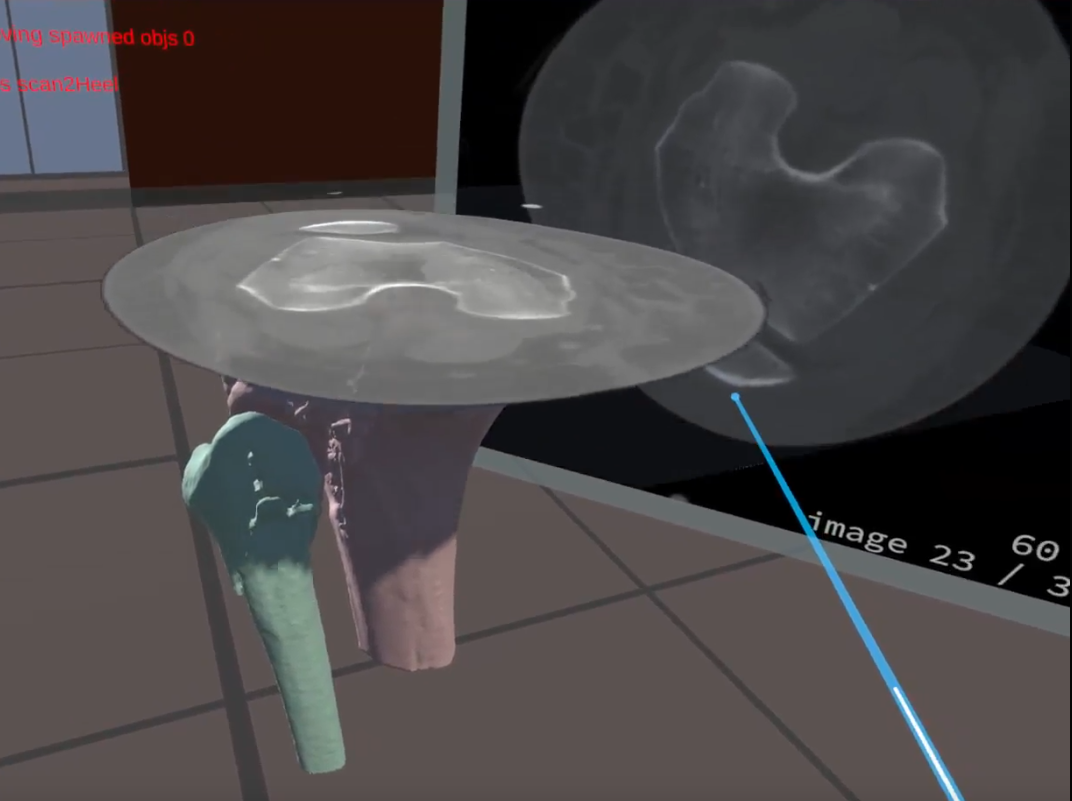
\includegraphics[height=180pt]{images/intersection.png}}
	\hfill
	\caption{CT intersection}\label{intersection}
  \small
  The selected CT slice is shown both in 2D and as a overlay on top of model. Notice that the upper part of the model is not rendered.
\end{figure}

When overlaying the slice texture onto the intersection plane, the image will completely obscure the model when looking down at the image. This removes the point of overlaying the CT image, so the picture is created as partially transparent. When the texture is created, the grey value is used as input for calculating the transparency of the pixel. This results in most of the outside of the image being completely transparent.

\subsection{Implants}

\begin{figure}[h!]
    \centering
	\subfloat[][]{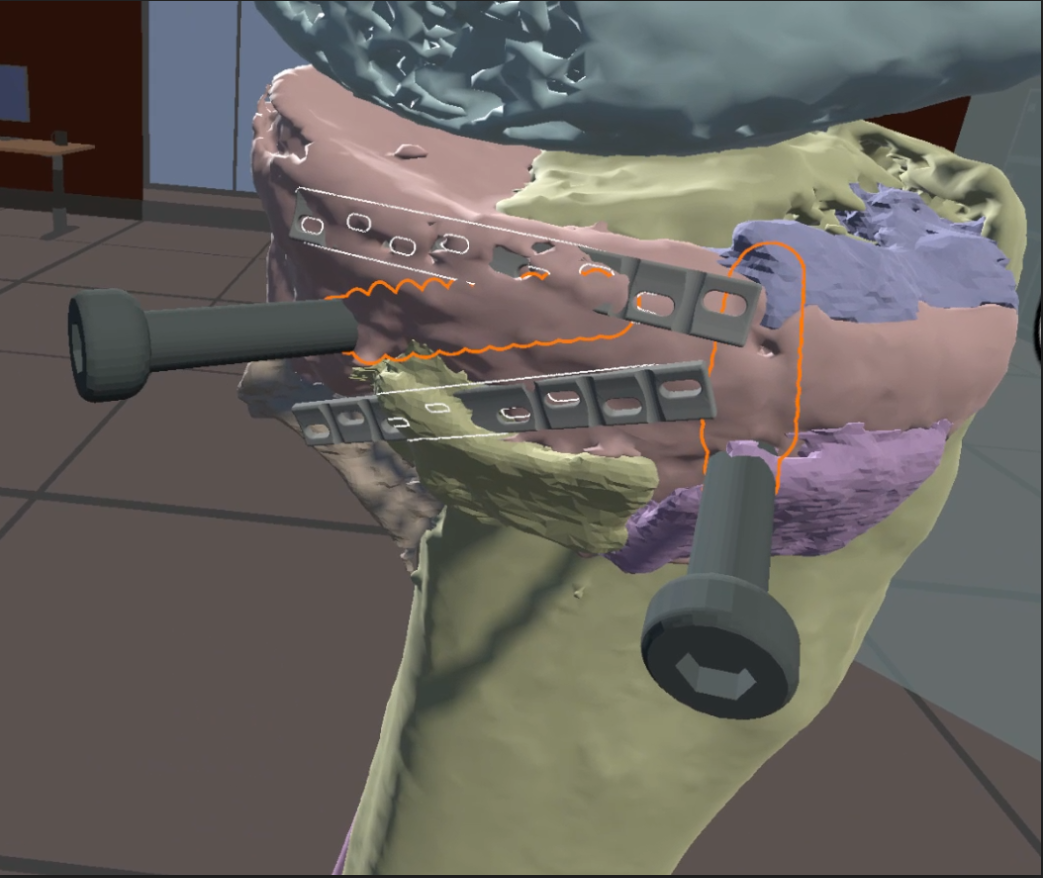
\includegraphics[height=180pt]{images/implants.png}}
	\hfill
	\caption{Implants}\label{implants}
  \small
  Picture showing 4 implants placed on and inside the fracture. Outline makes it easy to understand the exact position.
\end{figure}

The menu has a sub-menu for choosing what implant to add to the scene (figure~\ref{implantsmenu}). It consists of a list with a description and a preview of the implant. Pressing a button will spawn the selected implant in front of the user, and can then be moved in the same way a model part can be moved.

To improve the surgeon's ability to line up screws and find what parts of the fracture is penetrated by the screw/object an outline is shown as in figure~\ref{implants}. This allows the user to see where an object is compared to any other parts, even if it is entirely obscured by the model. This is achieved by a shader using a depth buffer to only draw the outline when obscured by other meshes~\cite{technologies_unity_nodate-1}.

\begin{figure}[h!]
    \centering
	\subfloat[][]{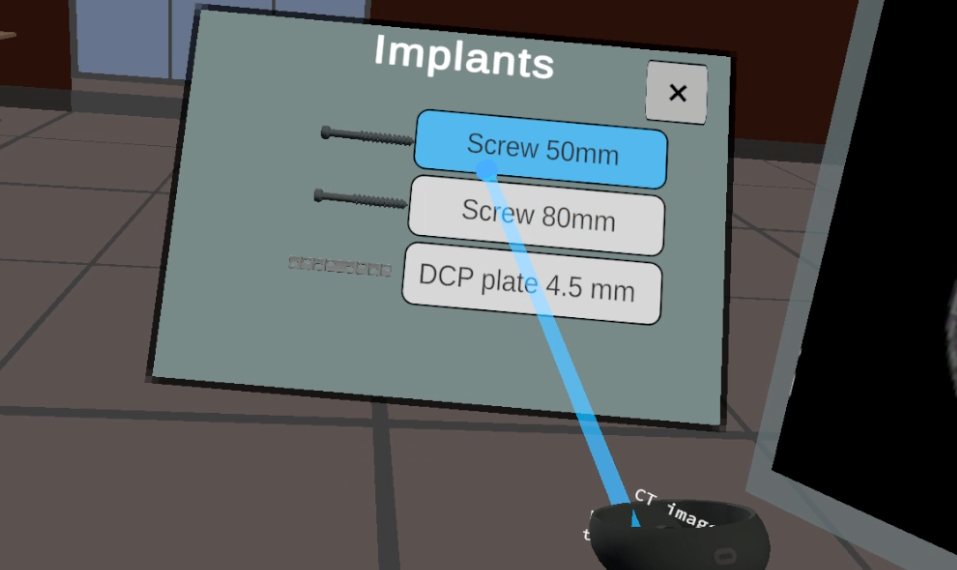
\includegraphics[height=180pt]{images/implantmenucrop.png}}
	\hfill
	\caption{Implants menu}\label{implantsmenu}
  \small
  The menu used for selecting implants, with a side by side preview.
\end{figure}

\section{Performance}
Performance guidelines for Occulus Quest hardware are outlined by the Occulus developers for the Quest 1 in the documentation~\cite{noauthor_oculus_nodate}.

The recommended triangle count is between 350k and 500k triangles~\cite{noauthor_performance_nodate}. The imported meshes can have a high vertex count and are reduced manually using remeshing in MeshLab~\cite{cignoni_meshlab_2008} to bring the total to under 500k. The reduced quality is barely noticeable when viewed in the resolution of the Quest HMD.
The mesh simplification could be automated, but this limit would be irrelevant if using a headset with a modern GPU for dedicated rendering.

TODO: performance data?


\chapter{Results and Discussion}

User tests were performed during and after the project to evaluate the application and try to answer the research questions. In this chapter, the tests and the results are described.

\section{Evaluation}

%SUS intro
System Usability Scale~\cite{system_usability_scale_sus_system_2013} (SUS) was used to get quantitative data to be able to compare between user groups or make conclusions on usability.
The survey consists of 10 standardized questions that are answered on a scale on 1 to 5. The questions are translated into Norwegian and are available in the appendix.

The survey was answered by 3 orthopedic surgeons, 3 professors in radiology or radiography and 2 radiography students. The total participant count of 8 is high enough to give a good indication of program usability~\cite{experience_why_nodate}, being measured to 75 \% accuracy in a specific study~\cite{tullis_comparison_nodate}.


\subsection{Participants}

For evaluating the surgery planning use case, the application was tested on two orthopedic surgeons currently working at Haukland University Hospital.
%experience
Both surgeons had more than ten years of experience in orthopedics and claimed to be very proficient at reading CT images and recognizing fractures.
Both participants had limited experience with any virtual reality, rating their own experience at 3 out of 10.

Having only two participants means it is difficult to conclude the research questions fully. However, the semi-structured interview does provide considerable insight into the research question and is discussed later.

For evaluating the educational use case, the participants were both radiology and radiography professors and radiography students.

\subsection{First test}
Date: 16 Jan. 2022

This was the first test done with professional orthopedic surgeons. Previous to this test, only the surgeon on the team had proposed what functionality was needed in the product.

The goal was to determine if any of the proposed use cases and implemented features were relevant for end users and if any additional requirements was needed.
%approach

Before the test, the intended use cases were described to the participants. The intended use case was improving the understanding compared to traditional slice visualisation given a complex fracture.
Testing was performed by introducing the application and explaining how to use the VR controllers. Afterward, each surgeon would have 5 to 10 minutes to try out all features at their own pace. The HMD was mirrored to a screen to observe what the user was doing. Minimal guidance was given during the testing, except for clarifying questions on bugs or limitations.

\subsubsection{Results}
%observations
The participants struggled with the controls for the first two minutes, especially understanding what buttons to press and how to pick up model parts. After the initial struggle, the participants easily interacted with the program.

The application had no way of moving the entire model closer to the player and relied instead on the $Reset\ View$ button integrated on the Quest. It was hard to find and use this button for the user.

%kommentarer fra enkelte
After testing the application, the participants gave feedback on the functionality.
The model is missing data on bone density and all bones appear equal even if they have different densities. The bone density is relevant because only solid bones can be drilled into. The model is also lacking some info on bone mass because bone with density below a density threshold could have been ignoring when making the model.

The model pieces were in large segments and so smaller fracture parts could not be moved individually. Smaller pieces should have been movable in order to perform reduction on the fracture.

%general feedback
Both surgeons agreed that using VR to understand the fractures was a minor improvement from 2D and 3D models.
The reason stated was that both surgeons are very experienced with reading 2D CT images and can easily recognize a familiar fracture on CT images, often without any 3D model. Both suggest a use case for training or education where CT imaging is harder to read.


\begin{figure}[h!]
    \centering
  \makebox[\textwidth][c]{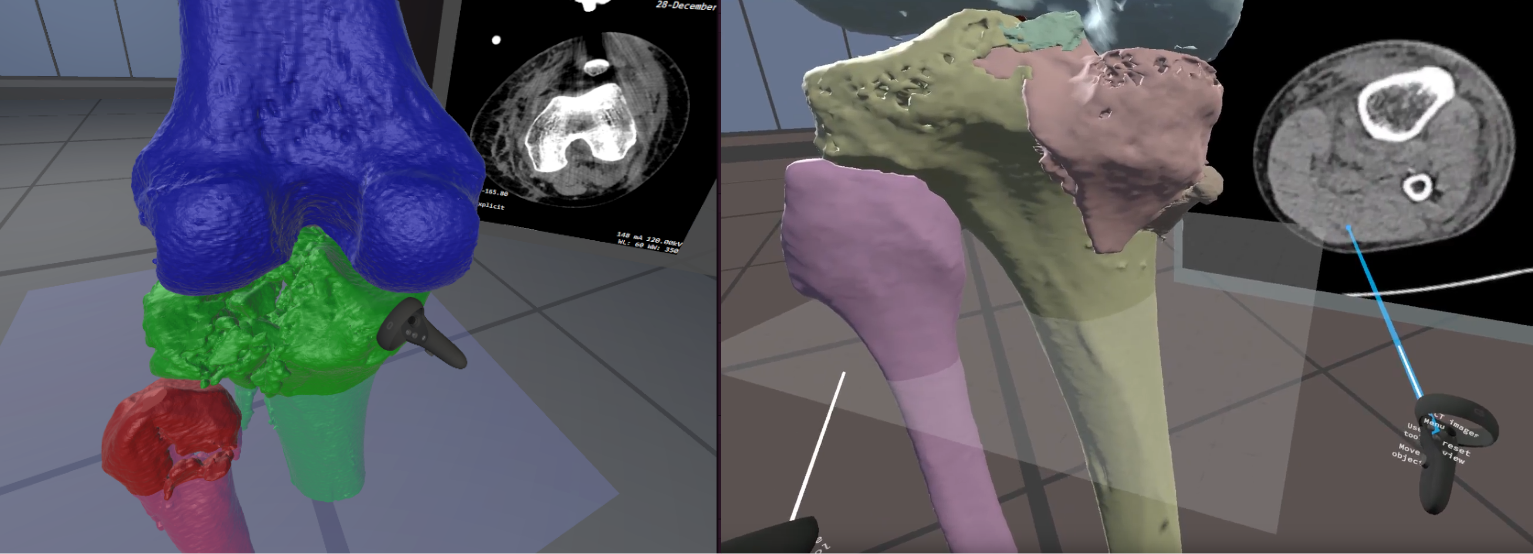
\includegraphics[width=0.8\textwidth]{images/test1and2.png}}%
	\hfill
	\caption{First and second test comparison}\label{test}
  \small
  visualisation changes on second test. The fracture part is split into several pieces and colors are less saturated.
\end{figure}

\subsection{Second Test}
Date: 5 May 2022

This test was done with the same orthopedic surgeons from the first test.
The goal was to evaluate how the final application could be used as a planning tool.

Between the first and second test the application was improved based on the previous results (Figure~\ref{test}).
A similar fracture to the first test was split up into three times as many smaller individual pieces to allow for reduction planning.
Implants was also further developed.
Other miscellaneous changes were added to improve the user experience.

The approach to this test was similar, except for a more structured evaluation. After the participants finished testing, a semi-structured interview, including System Usability Scale questions, was done.


\subsubsection{Results}
%observasjoner
As the surgeons had tried an earlier version, they quickly got used to the controls, even with four months between tests. 
Manipulating the model seems easy and requires no guidance. The functionality that is available in other programs, such as scaling/zoom, rotation and CT images was familiar and easy to use.

Some of the application design did not work out as expected.
When rotating the model, one participant tried to rotate on another axis, but only z-axis rotation is supported. Viewing the model from the z-axis (top down view) is common in other viewers.
The application had no way of resetting the model position, sometimes causing the user to reach into a wall or furniture. There is also no way of picking up a model physically out of reach.

When using the measurement tool the user is expected to place new points to reset the previous measurement. One user tried moving the measurement points similarly to the grabbable objects, which resulted in some confusion.

%enkelte kommentarer
One participant mentioned that using controllers to manipulate tilt and rotation is easier with VR controllers compared to mouse and keyboard. This is relevant for planning with implants.

A participant said moving model parts for planning surgery is seldom relevant as bones are often moved very short distances. Bones are attached to soft tissue, and moving them is very restricted.
Also the surgeon almost always knows where fracture parts are supposed to be, and does not need to plan the movements. There is however, exceptions to this with specific complicated fractures.

Measurement tools are helpful, as they are also used in traditional programs, and missing them would be a disadvantage.

%feedback
The general feedback is that the benefit from visualising in VR is pretty insignificant in almost all cases, as the information gained from 2D images and 3D models is sufficient.
This is mainly due to experience and how easy it is for surgeons to recognize a familiar fracture. Often the surgeon has performed the same type of surgery 100+ times and only needs to recognize the type of fracture. Additionally, creating the required 3D model makes the benefit less significant.
There is a slight improvement in visualisation, but it may not be worth creating a 3D model and using a HMD to view the model.

%TODO: sammenlignet med 3d printing
A participant said when comparing to 3D printing that he rarely requested prints, of the same reasons mentioned earlier: When viewing CT images he very often recognizes a familiar fracture.

%Knut feedback
Some of the interview results are from the surgeon on the team that was included in the development process. He could be biased on how easy the software is to use or on how useful it is, but is still included for sake of discussion.

TODO: knut interview

%SUS result ortopeder
The result from the SUS questions was 58.75 points out of 100 (n=2), which places it at OK~\cite{bangor_empirical_2008}. The sample size is too small to conclude anything, but the result can still be a topic of discussion. The questions used and average scores are available in the appendix.

\subsection{Radiograph testing}
Date: 16 - 20 May 2022

The application was tested on radiograph students on HVL to explore any education benefits. Only two students participated. The students had completed 2 years of the radiograph bachelor and had some experience with interpreting CT images and had been using VR for anatomy education. The VR program used at HVL is called 3D Organon~\cite{organon_3d_nodate}.
The existing VR program they used was an anatomy model and did not include any CT images or fractures.
It was also tested on three professors in the radiography course at HVL.
The testing was performed in a similar way, but with education and CT image interpretation as a goal.
Both students and professors also answered the SUS form.

\subsubsection{Results}
%student feedback
The students had no trouble with using the application or VR in general. They discovered controls and features without any additional guidance. They also gave feedback on the application being very easy to use and intuitive.

The students agreed the tool was a good educational tool for learning CT image interpretation, especially early in the study programme.
One participant said viewing the height of the selected CT slice made it easier to understand the image.

One student mentioned moving the fracture parts was useful to understand what a fracture looks like.

A suggestion was to use labeling for the CT images, as used in existing tools. The labeling could show bone names or other points of interest. It could also be shown on both model and the images.

An educational tool should preferably include other body parts and include soft tissue data. Especially heart or brain is difficult to understand.


% testing av professorer
The professors interviewed teaches in different courses at the radiography bachelor, and all have a radiograph or radiology background. 
All participants has previously used similar VR tools at HVL.

They agreed students lack some skills in interpreting CT images. This is caused by a lack of training during the courses and in practice at hospitals. Using a tool that helps with understanding CT images would be valuable. 

The existing VR tool they use at HVL does not contain CT images or fractures, so this application would substitute it well.

Similarly to the students, the professors required little to no guidance. Every participant said the application was easy to use or similar.

A participant said viewing the model and images side by side supplements each other, and is valuable for teaching students. Similar tools with a side by side view already exists, but VR makes it even better.

All participants mentioned a larger selection of data should be available, and one mentioned other scan types to include muscle or lungs. The larger dataset should preferably include the entire body.

On the question \emph{Should this be used in education?} one participant answered it has value but could be difficult to choose what is should replace, and they may not have any time available. Another said it fits in with existing use of VR, and will be even better as VR becomes more common and the students gets accustom to the technology.

%SUS result
The SUS score from educational users was 87.5 (n=5). Maximum score was 97.5 and minimum 72.5. The adjective rating is very good~\cite{bangor_empirical_2008} and is above the average SUS score of 68.





\section{Discussion}

\subsection{VR development}

The application had two design goals of being easy to use and give a good anatomy understanding.
There are some user experience errors apparent in testing that should be improved for better user interaction. The following points are identified as the most critical improvements:

The most important is handling Interactable objects physically out of reach. Some VR games use a ''force grab'' mechanic where grabbing a distant object moves it towards the users hand, which could have solved the issue.

Being able to move the model is a repeating issue. This includes adjusting the height to adjust for a sitting or standing position, or moving the model closer or further away if the user moves in real life. A similar issue is moving the model on other axis, to view from other angles. This feature would be nice to have as well as it is a source of frustration for some.
This issue does not have an obvious solution, as grabbing is reserved for another action and there is no available joystick controls to use. A proposed solution is using a modal solution and use grabbing in conjunction with a button press, but this increases complexity for users. Another could be automatic distance from user and automatic height based on user height, but moving objects without user interaction is considered bad practice. A final suggestion is a UI similar to the menu system to control movement.

Measurement worked fine for the users that understood the usage, which gave good feedback on being able to accuretly measure distance on several axis. The interface is differs itself from the rest of application because it uses button clicks and could have been reworked to a grab interaction.

Transparency was a much requested feature during testing. The reason was split, it could have used to show density or it could simply be used to view soft tissue layered on top of bone. It would definitely have been a nice feature, was had some technical limitations described previously. Had it been planned feature at the project start, the application could have used DICOM data to generate transparent volume data. Potential issues would be both performance and data segmentation, so the opaque models seems like a reasonable solution.


%hardware
As development and testing was done on a particular headset, hardware choice and limitations could have an impact on results. The Quest 2 is a fairly recent headset released in 2020~\cite{noauthor_oculus_nodate}, but is a cheap consumer headset with lower specifications than more expensive alternatives. This primarily affected how well the application could render large datasets without lagging.
Testing could potentially have compared headsets with different resolutions and performance to find if this causes a worse user experience.
Virtual Reality and Augmented Reality is fields with a lot of development, and future hardware will probably make VR or AR an even better alternative.

\subsection{Evaluations} %discussion
%Testing orthopedic
This result on the surgery use case describes what experienced surgeons that are very familiar with current tools think of VR. They have little VR experience and do not use VR regularly. One can assume this increases scepticism compared to students using VR almost daily.

%SUS begrunne
The SUS scores gathered total 8 answers, divided between the fields of orthopedics and radiography.
The SUS participant count for each user group is low, but the total of 8 is high enough to give a good indication of the usability. It should be noted that the total SUS score is an average from several roles that view the application from different perspectives. Testing distinct user groups is both a benefit as it is more thoroughly tested, but makes it harder to conclude on usability for a specific user base.

%SUS om ortopeder
The SUS score from surgeon testing of 59 indicates a less than average application usability, which is 68~\cite{system_usability_scale_sus_system_2013}. The low usability score is plausibly skewed by scepticism towards the use-case and not just the user experience of the application itself. The question \emph{I want to use the application often} had the lowest possible score of 1/5 because of what tools they already use are sufficient, and not because of the applications usability. This questions does however imply that the application is not very useful for experienced surgeons.

%Compared to existing tools
Comparing the VR viewer to the existing 2D and 3D tools in Materialise used at Haukland University Hospital, there are definitely advantages.

Potential advantages are related to controller manipulation and depth perception. Rendering with depth is likely not useful for experienced surgeons, but is promising for less experienced surgeons.
Controllers could be beneficial for complex planning of surgeries because of the easy 3D manipulation.

%sammenligne med 2d og printing
VR has some obvious benefits over 3D printing such as digital tools and more complex visualization.
However an important question is whether to compare VR to just 3D printing or printing in addition to 2D tools. As 2D tools are often used together with 3D printing, VR should be compared to both. Some advantages to VR like transparency or cross sections is also available in 2D applications.

Tools like measurement already exist in current 2D tools. The similar tools in VR gives few benefits except for better controller manipulation when placing or moving objects.
Controller manipulation seemed to be the best advantage but did not have many practical use cases, according to interviews.
Implants have some advantages when digital, such as 'screwing' in a screw, and then resetting the model. Implants can also be adjusted and manipulated digitally without having a physical model.

3D printing has some advantages hard to recreate in VR. The first is physical touch, which controllers can not reproduce. Another is accurately using tools or implants with the model, which can be simulated, but with a lower precision than real life.

%remote
VR has the advantage of remote usage or remote cooperation, which is very limited with physical prints. This has however not been tested in this project. It is obvious that multiplayer and remote usage is possible as there are many such VR applications.

%Education
The response from the educational point of view was very good. They already use similar VR tools, so the barrier to picking up such a tool is fairly low.
As the educational purpose was not the original use case for the project, it is not designed with any teaching tools in mind. There is, however, very few features requested that would be specific for educational purpose. The only example is labeling of body parts. 
Using such a tool in education is very promising, and during this project the radiography department has been very interested in its uses.
%general benefits
VR has documented benefits in learning and education. The benefits is likely to apply when using the application for this use case.

TODO: SUS om education
The SUS score of 87.5 is significantly higher than the surgeons giving a score of 59.
The participant count of 5 is low, but gives some insight on usability. With a lowest score of 72, it is clear education was a more reasonable target group based on SUS results. The good score also reinforces the positive feedback in interviews.

%konklusjon applikasjon
The final application is overall working well and mostly accomplishes the first design goal of being easy to use. The ease of use is important in order to evaluate the research questions, as a cumbersome application would influence the feedback on how useful VR is.
The other goal of giving users a good understanding of the fracture is partly met, VR gives some benefits to visualisation, but it is a small increase compared to existing tools.
The test participant surgeons does not believe it helps much in surgery planning. It has advantages over 3D printing, but the participants rarely uses printing anyways. It has a lot of potential in complex fractures where printing is limited and the fracture is hard to understand, but these kind of cases are rare.
The student participants have different opinions and benefit a lot more from VR visualization in educational purposes. The different opinion between experienced surgeons and students could be caused by different medical fields, radiology experience, age or intended use, or a combination.





\chapter{Conclusion}
Given the evaluation results described earlier, we try to answer the proposed research question by looking at the two sub-questions:

\section{How VR can improve surgery planning}

With experienced surgeons as the target group, there was no indication of VR itself improving the quality of the planning and improving the outcome of the surgery.

%3D printing
It is established that VR is a technology that requires fewer resources compared to 3D printing. In the context of surgery planning, it seems VR can give the same advantages as 3D printing, making it a feasible alternative. However, as both have unique advantages, VR can not be considered a complete replacement.

\section{VR for CT interpretation education}
There are studies showing the usefulness of VR in education and how it benefits motivation and learning outcomes. This benefit in addition to the different visualization VR brings makes VR a great addition to medical imaging education.

Even with a small sample size, both students and professors expressed great interest in the application. It is therefore likely that VR is a good tool for education in CT interpretation and fracture anatomy.



\chapter{Further Work}
This project would require more testing for it to be reliable. Testing should include a higher sample size and broader demography of specializations, ages, and experience.

\section{Educational Tool}
As this project was tested as a educational tool with good results, it could be developed further. The application does not contain any tools directed towards teaching. This use case probably has some potential not fulfilled by this application.

\section{Other fields}
There are many other medical fields beside orthopedics that use radiology for diagnosis and planning.
CT, MRI, PET and ultrasound can all produce image slices and 3D models, and these could be visualized with a very similar application, especially anything using the standard DICOM format.
Examples are neurosurgery or cardiovascular surgery that typically use MRI scans instead of CT, and also require some planning in advance.

TODO: lage alt dynamisk, automatiske datasett, oppdatere CT bilder automatisk

\section{Education}


\appendix
\chapter{Source code} \label{SourceCode}

The source code for the VR application is available at this URL: \url{https://github.com/tobias2912/VR-DICOM-viewer}.


\begin{figure}[h!]
    \centering
  \makebox[\textwidth][c]{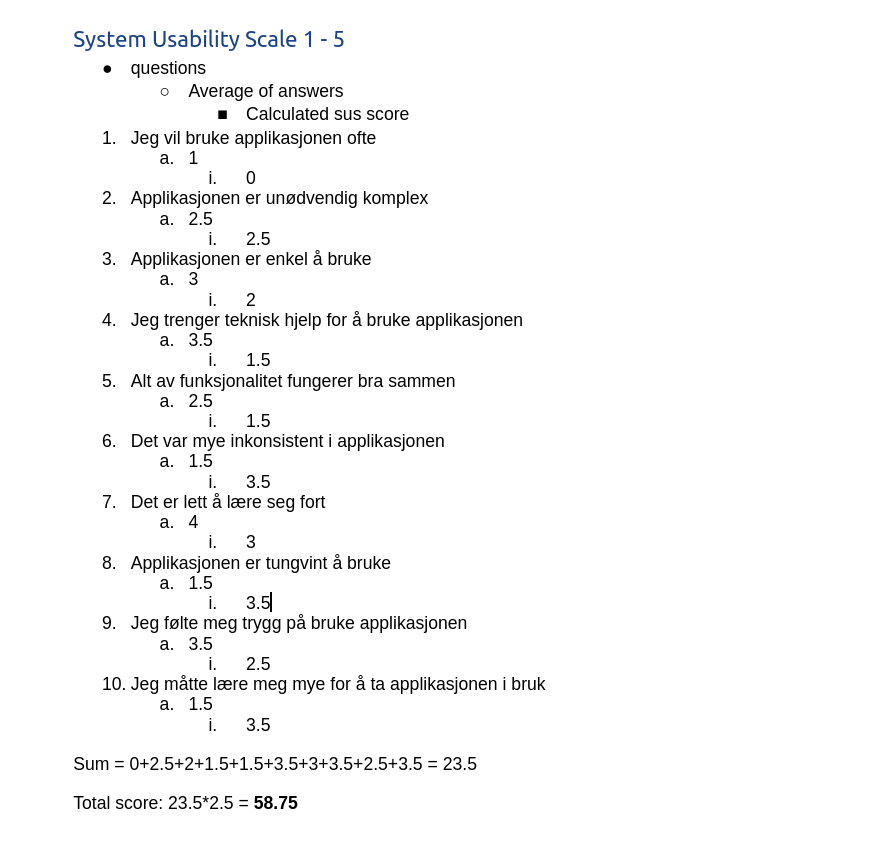
\includegraphics[width=1.3\textwidth]{images/sus.png}}%
	\hfill
	\caption{SUS scores}\label{sus}
  \small
\end{figure}

\begin{figure}[h!]
    \centering
  \makebox[\textwidth][c]{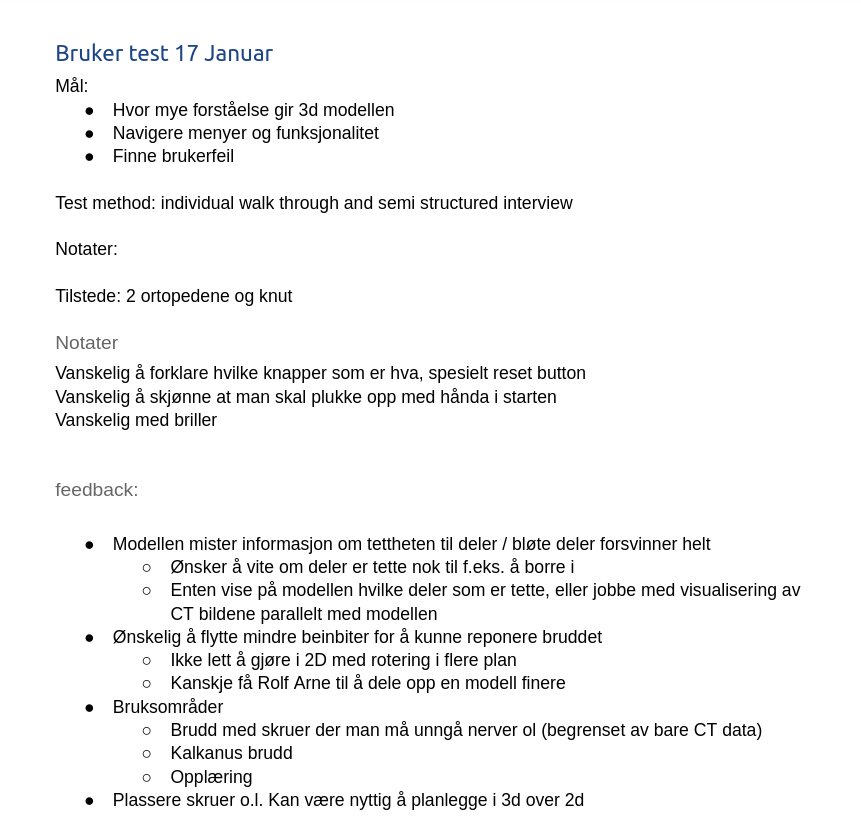
\includegraphics[width=1.3\textwidth]{images/intervju1.png}}%
	\hfill
	\caption{Interview notes from evaluation}
  \small
\end{figure}

\begin{figure}[h!]
    \centering
  \makebox[\textwidth][c]{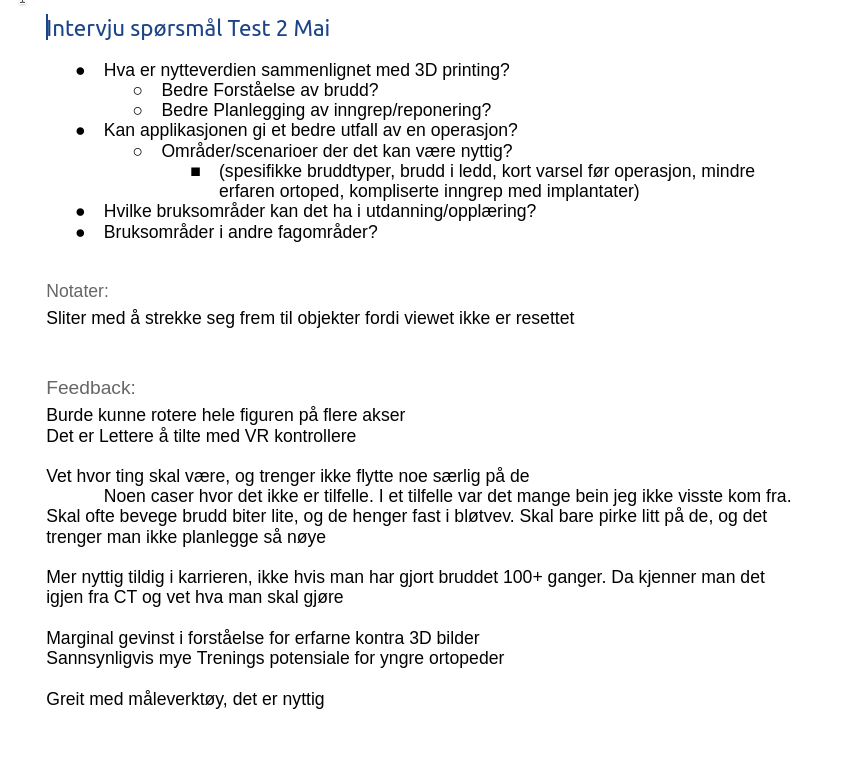
\includegraphics[width=1.3\textwidth]{images/intervju.png}}%
	\hfill
	\caption{Interview notes from evaluation}
  \small
\end{figure}
%\bibliographystyle{splncs04}
%\bibliography{references}
\printbibliography

\end{document}
